\documentclass[12pt]{article}
\usepackage{fontspec}
\usepackage{graphicx}
\usepackage{geometry}
\usepackage{float}
\usepackage{hyperref}
\usepackage{polyglossia}
\setmainlanguage{farsi}
\setotherlanguage{english}
\newfontfamily\englishfont{Times New Roman}
\newfontfamily\persianfont[Script=Arabic]{XB Zar.ttf}




\geometry{a4paper, margin=2.5cm}
\usepackage{setspace}
\onehalfspacing
\usepackage{titling}
\usepackage{etoolbox}
\usepackage[backend=biber,style=numeric,sorting=none]{biblatex}
%%%%%%%%%%%%%%%%%%%%%%%%%%%%%%%%%%%%%%%%%%%%%%%%%%%%%%%%%%%%%%%%%%%%%%%%%%%%%
\makeatletter
\newcommand{\persiandigit}[1]{%
	\ifcase#1 ۰\or ۱\or ۲\or ۳\or ۴\or ۵\or ۶\or ۷\or ۸\or ۹\fi
}
\DeclareFieldFormat{labelnumber}{\persiandigit{#1}}
\makeatother
%%%%%%%%%%%%%%%%%%%%%%%%%%%%%%%%%
\newcommand{\persianordinal}[1]{%
	\ifcase#1
	\or اول%
	\or دوم%
	\or سوم%
	\or چهارم%
	\or پنجم%
	\or ششم%
	\or هفتم%
	\or هشتم%
	\or نهم%
	\or دهم%
	\or یازدهم%
	\or دوازدهم%
	\or سیزدهم%
	\or چهاردهم%
	\or پانزدهم%
	\or شانزدهم%
	\or هفدهم%
	\or هجدهم%
	\or نوزدهم%
	\or بیستم%
	\else #1\fi
}

\newcommand{\persianordinalpage}{\persianfont\persianordinal{\value{page}}}


%%%%%%%%%%%%%%%%%%%%%%%%%%%%%%%%%%%%%%%%%%%%%%%%%%%%%%%%%%%%%%%%%%%%%%%%%%%%%
\begin{filecontents}{\jobname.bib}
@online{gnu-coreutils-cut,
    author    = {{GNU Project}},
    title     = {cut invocation},
    year      = {2024},
    url       = {https://www.gnu.org/software/coreutils/manual/html_node/cut-invocation.html},
    note      = {Accessed: 2025-07-28}
}

@online{gnu-coreutils-head,
    author    = {{GNU Project}},
    title     = {head invocation},
    year      = {2024},
    url       = {https://www.gnu.org/software/coreutils/manual/html_node/head-invocation.html},
    note      = {Accessed: 2025-07-28}
}

@online{gnu-coreutils-tail,
    author    = {{GNU Project}},
    title     = {tail invocation},
    year      = {2024},
    url       = {https://www.gnu.org/software/coreutils/manual/html_node/tail-invocation.html},
    note      = {Accessed: 2025-07-28}
}

@online{gnu-coreutils-touch,
    author    = {{GNU Project}},
    title     = {touch invocation},
    year      = {2024},
    url       = {https://www.gnu.org/software/coreutils/manual/html_node/touch-invocation.html},
    note      = {Accessed: 2025-07-28}
}

@online{gnu-coreutils-wc,
    author    = {{GNU Project}},
    title     = {wc invocation},
    year      = {2024},
    url       = {https://www.gnu.org/software/coreutils/manual/html_node/wc-invocation.html},
    note      = {Accessed: 2025-07-28}
}

@online{gnu-coreutils-kill,
    author    = {{GNU Project}},
    title     = {kill invocation},
    year      = {2024},
    url       = {https://www.gnu.org/software/coreutils/manual/html_node/kill-invocation.html},
    note      = {Accessed: 2025-07-28}
}
\end{filecontents}

\addbibresource{\jobname.bib}

\defbibheading{bibliography}[]{%
	\begin{RTL}
		\section*{مراجع}
	\end{RTL}
}

%%%%%%%%%%%%%%%%%%%%%%%%%%%%%%%%%%%%%%%%%%%%%%%%%%%%%%%%%%%%%%%%%%%%%%%%%%%%%

\begin{document}
	
	% ==============================
	% Title Page
	% ==============================
	\begin{titlepage}
		\centering
		\vspace*{1cm}
		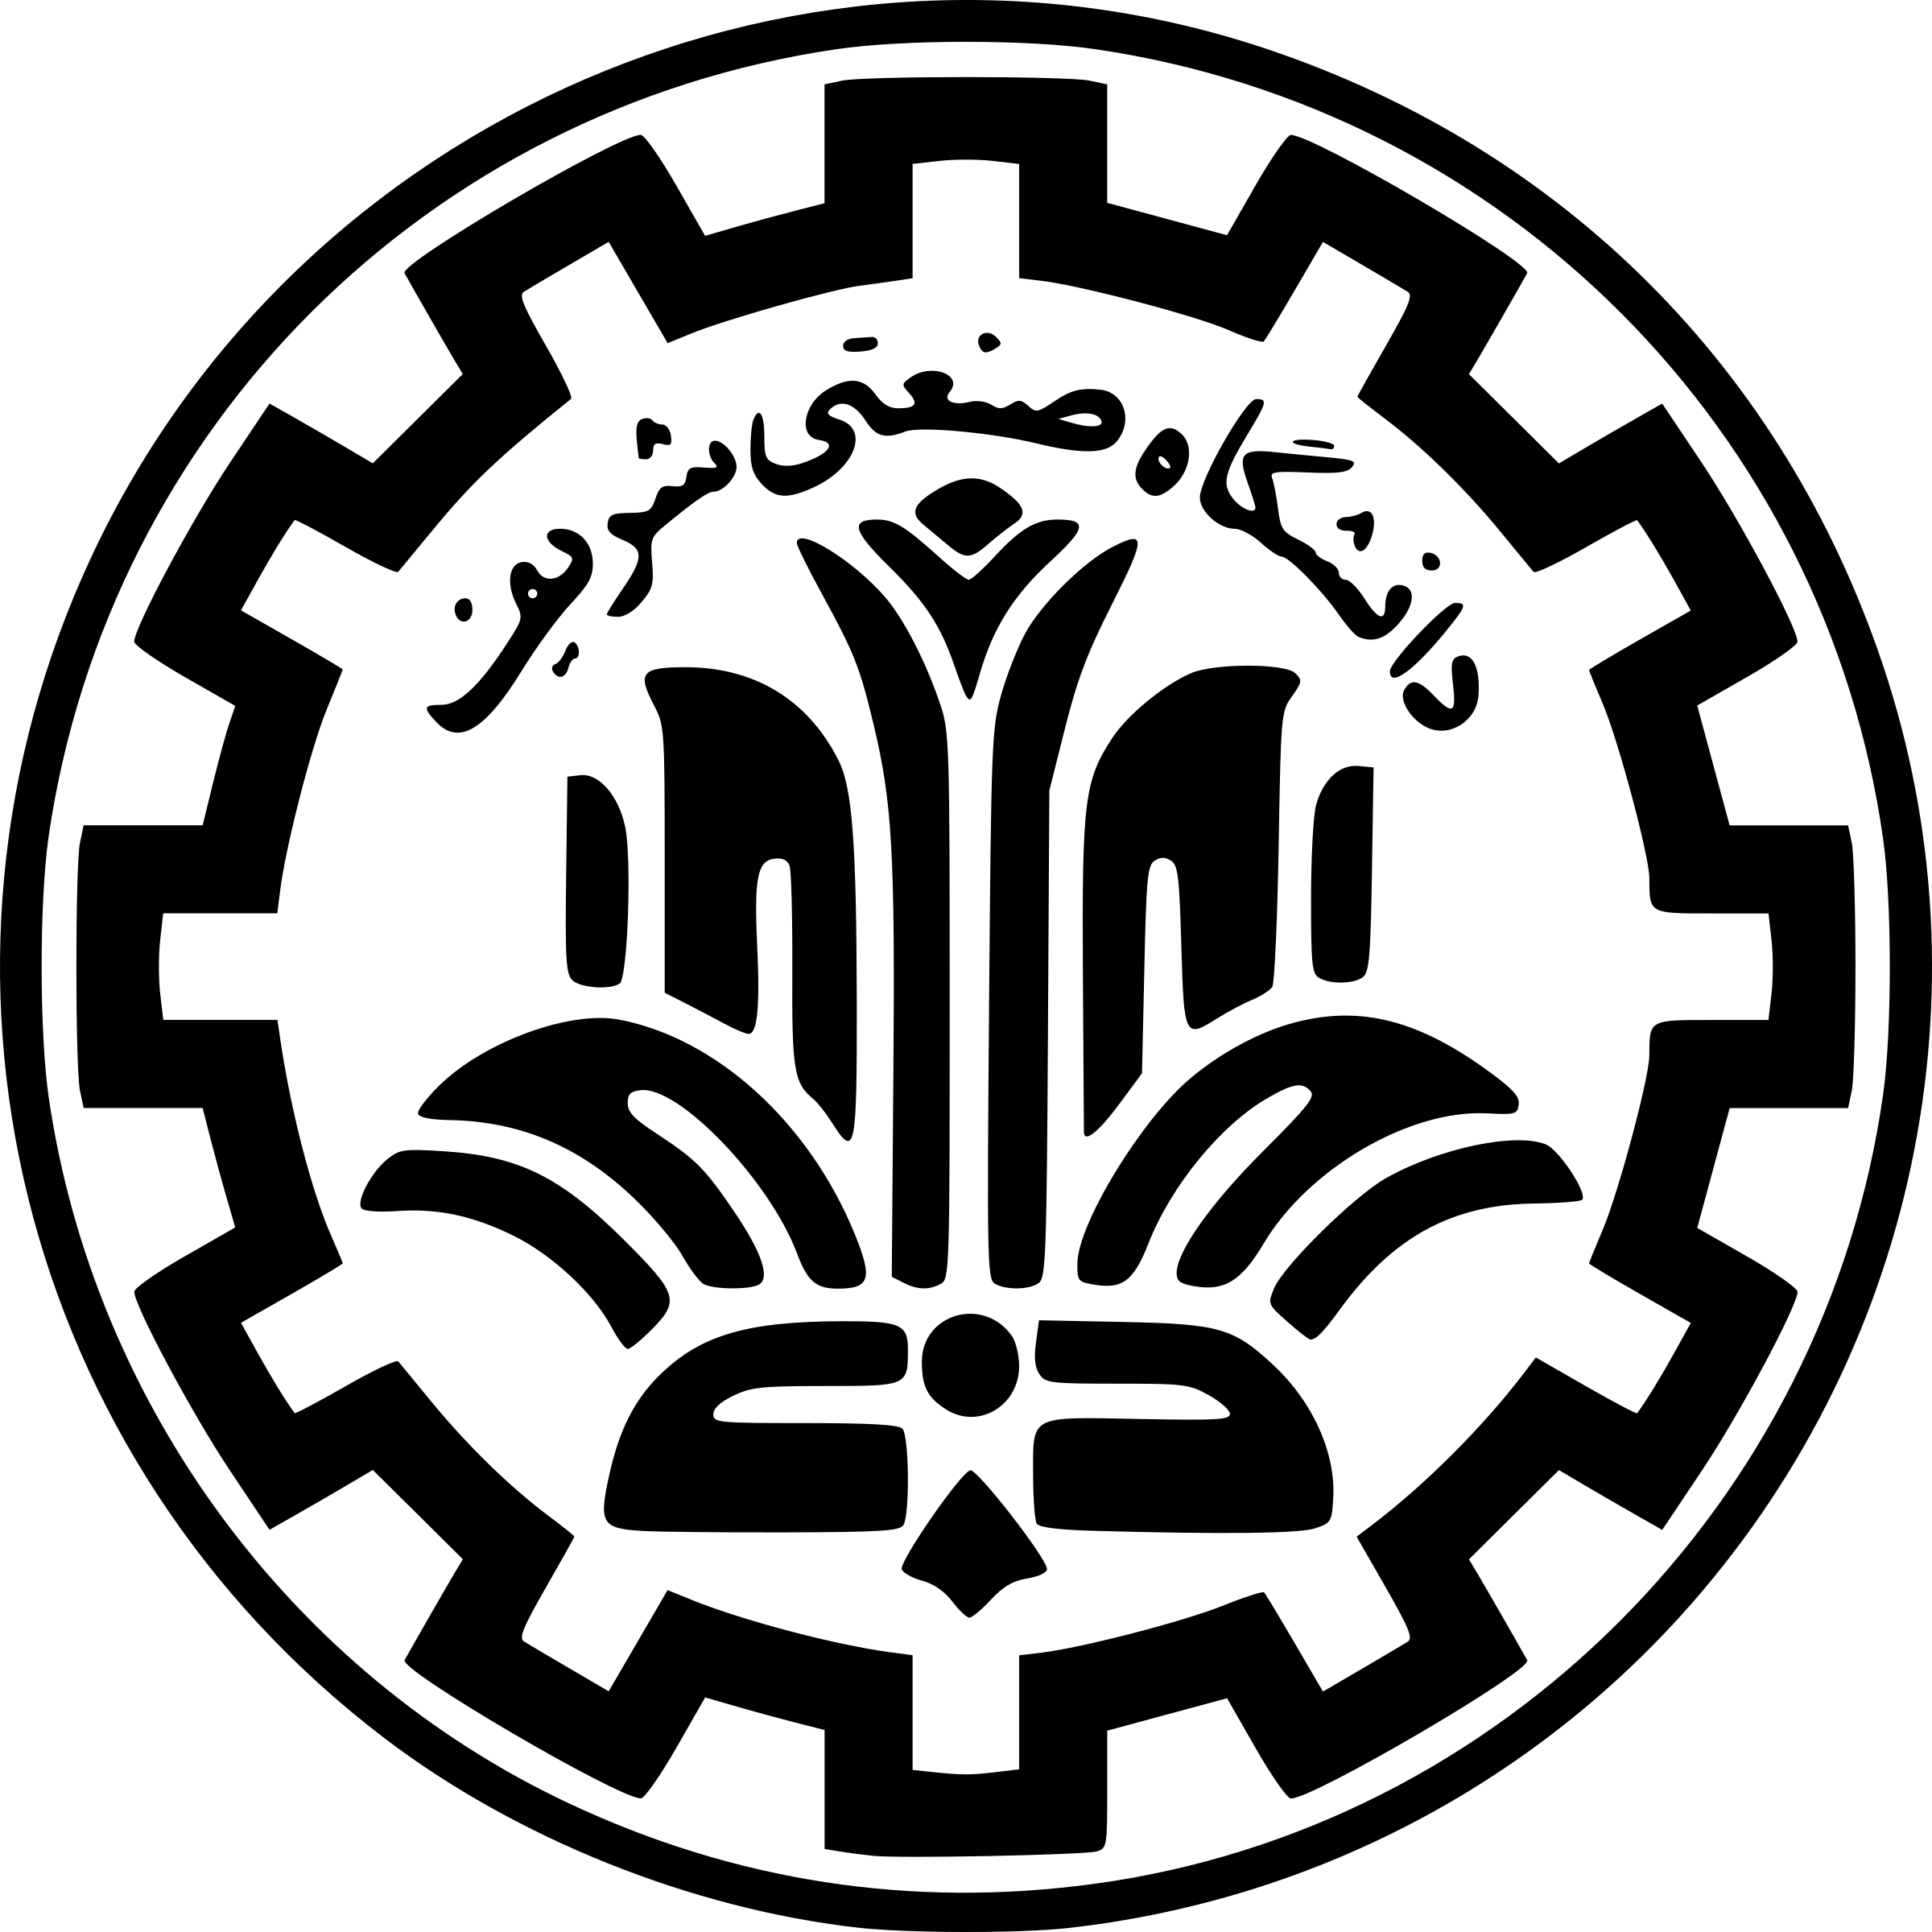
\includegraphics[width=4cm]{sharif.png}\\[1.5cm]
		{\Large\textbf{دانشگاه صنعتی شریف}}\\[0.5cm]
		{\large\textbf{دانشکده‌ی مهندسی کامپیوتر}}\\[1.5cm]
		{\Huge\textbf{گزارش کار آزمایشگاه}}\\[0.5cm]
		{\LARGE\textbf{آزمایشگاه سیستم‌های عامل}}\\[2cm]
		
		\textbf{گزارش آزمایش شماره ۱}\\
		(آشنایی با سیستم عامل لینوکس)
		
		\vfill
		\begin{tabular}{rl}
			\textbf{شماره‌ی گروه:} & ۲۰ \\
			\textbf{گروه:} &
			ارشیا یوسف‌نیا (۴۰۱۱۱۰۴۱۵) \\
			& محمدعارف زارع زاده (۴۰۱۱۰۶۰۱۷) \\
			\textbf{استاد درس:} & دکتر بیگی \\
			\textbf{تاریخ:} & تابستان ۱۴۰۴ \\
		\end{tabular}
	\end{titlepage}
	
	% ==============================
	% Persian Ordinal Page Numbering
	% ==============================
	\clearpage
	\setcounter{page}{1}
	\renewcommand{\thepage}{\persianordinalpage}
	
	\tableofcontents
	\clearpage
	\listoffigures
	\clearpage
	\listoftables
	
	% ==============================
	% Switch to Persian Digits (۱, ۲, ۳, ...)
	% ==============================
	\clearpage
	\setcounter{page}{1}
	\pagenumbering{arabic}
	\renewcommand{\thepage}{\persianfont\arabic{page}}
	
	
	% ==============================
	% Main Content
	% ==============================
        \section{شرح آزمایش}
        \subsection{نصب سیستم عامل لینوکس}

        \begin{enumerate}
            \item 

        ما از نرم افزار 
        \textenglish{VirtualBox}
        برای مجازی‌سازی سیستم عامل استفاده می‌کنیم. به دلیل منسوخ شدن 
        \textenglish{Debian8}
        مطابق نکته‌ی گفته شده در کوئرا، از 
        \textenglish{Ubuntu 24.02}
        استفاده می‌کنیم. در تصاویر زیر تنظیمات و مراحل راه‌اندازی را می‌توانید مشاهده کنید:
    
	
	\begin{figure}[H]
		\centering
		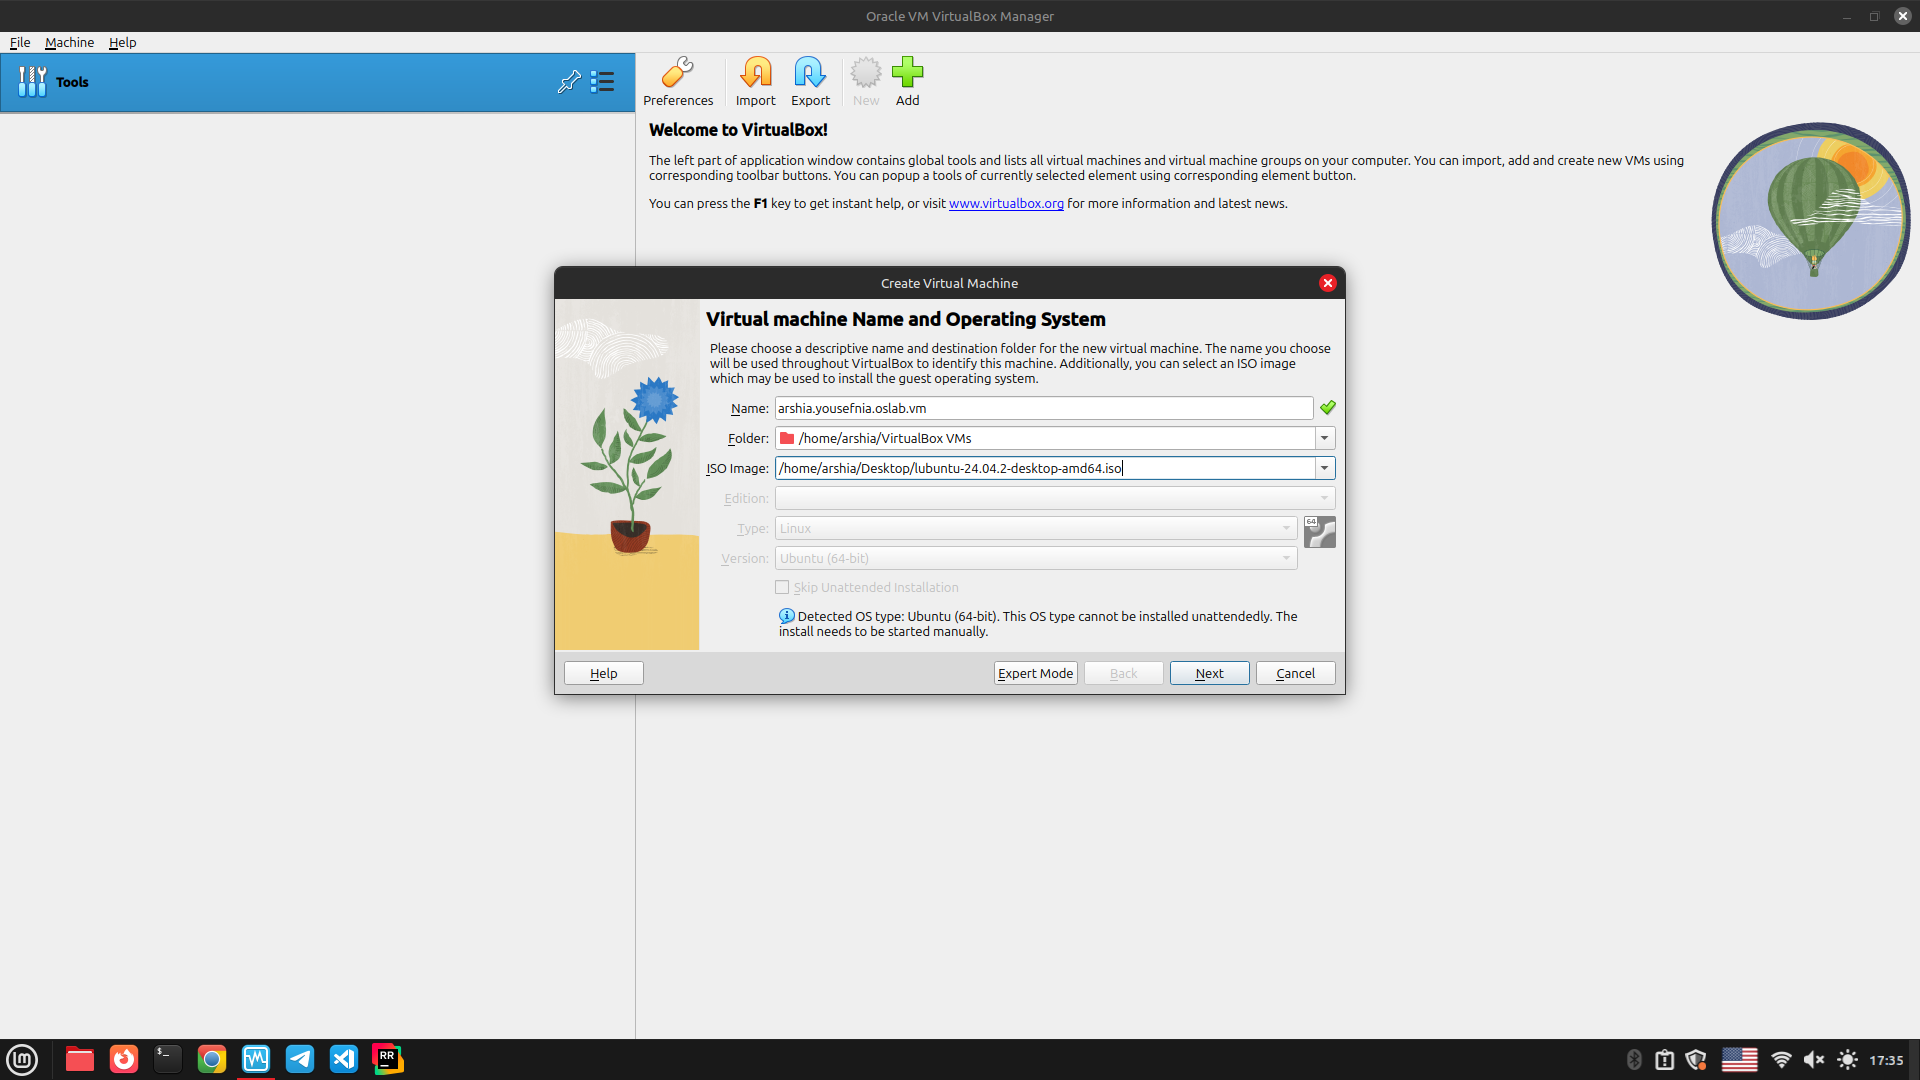
\includegraphics[width=0.8\textwidth]{report1-resources/1.png}
		\caption{انتخاب \textenglish{ISO Image} مربوط به \textenglish{Ubunto 24.02}}
	\end{figure}

        \begin{figure}[H]
		\centering
		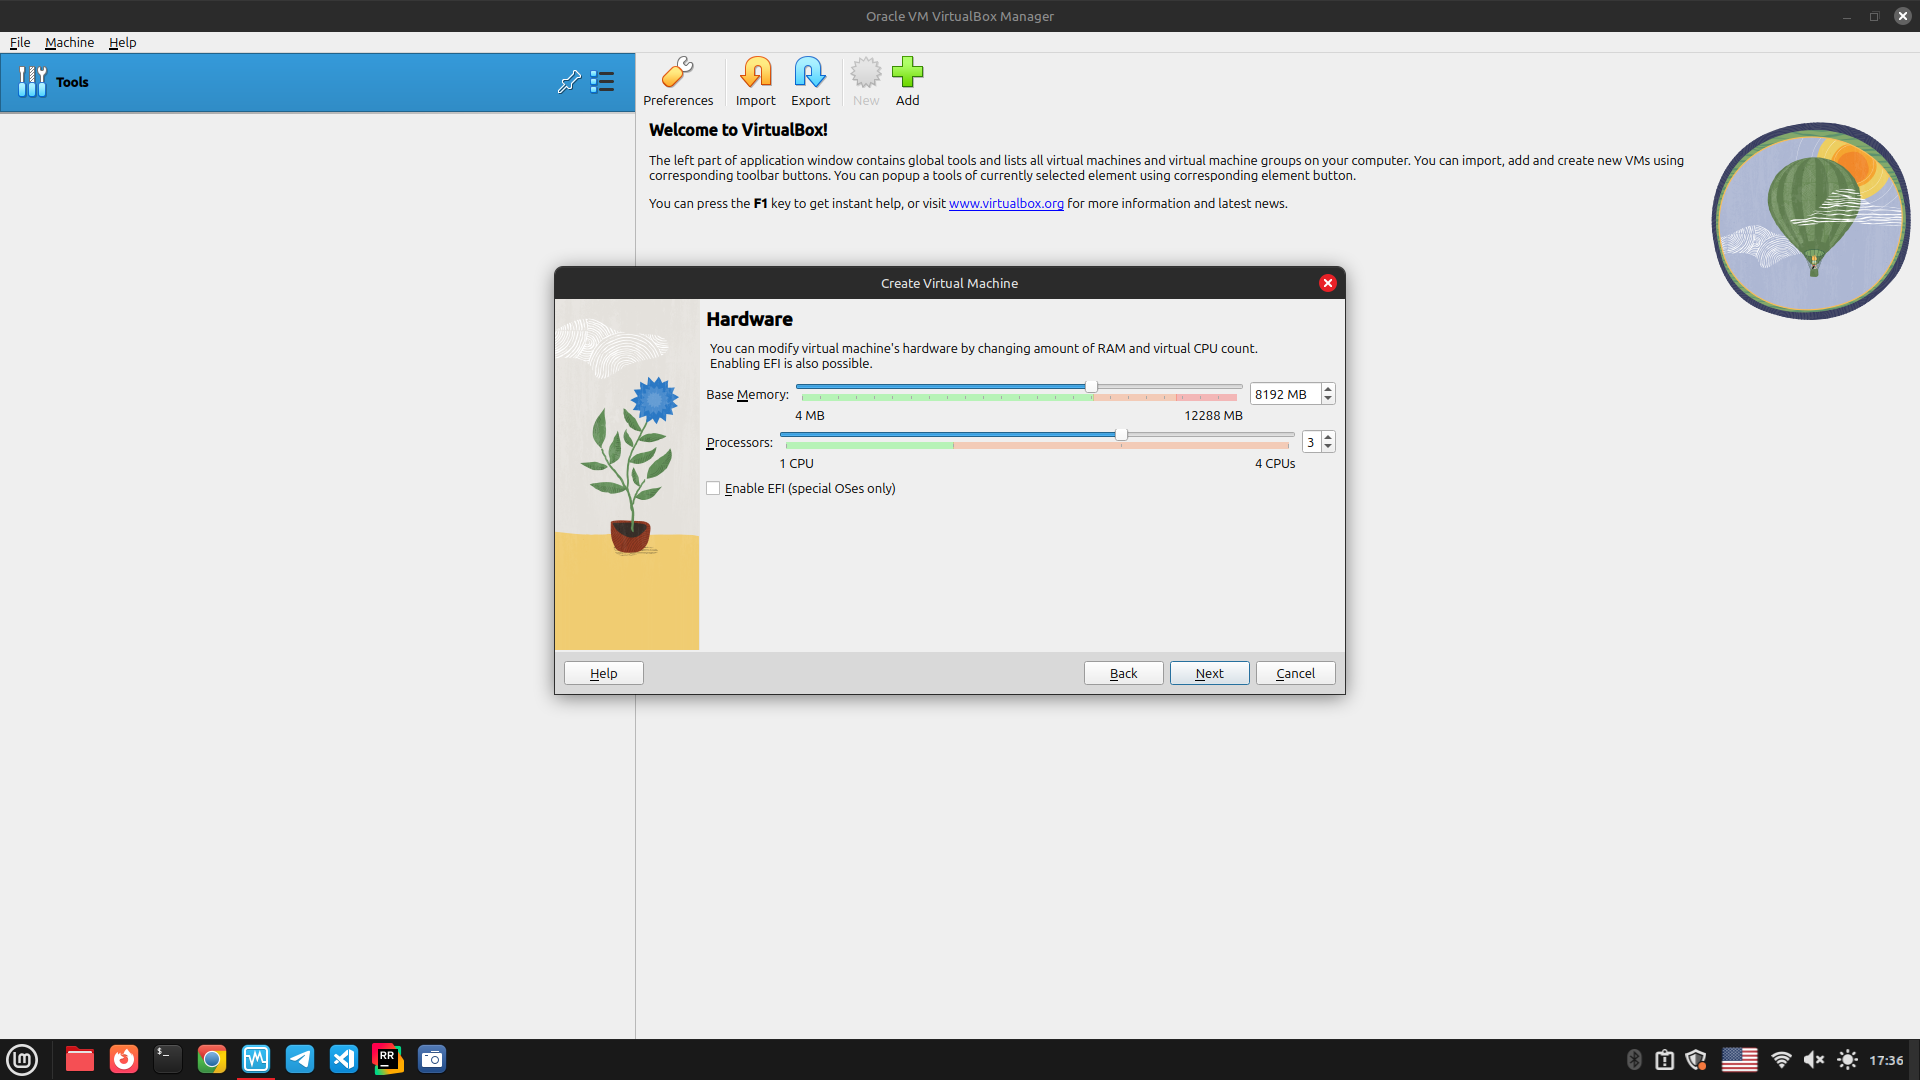
\includegraphics[width=0.8\textwidth]{report1-resources/2.png}
		\caption{انتخاب میزان دسترسی سیستم عامل مجازی به حافظه و پردازنده‌ها}
	\end{figure}

        \begin{figure}[H]
		\centering
		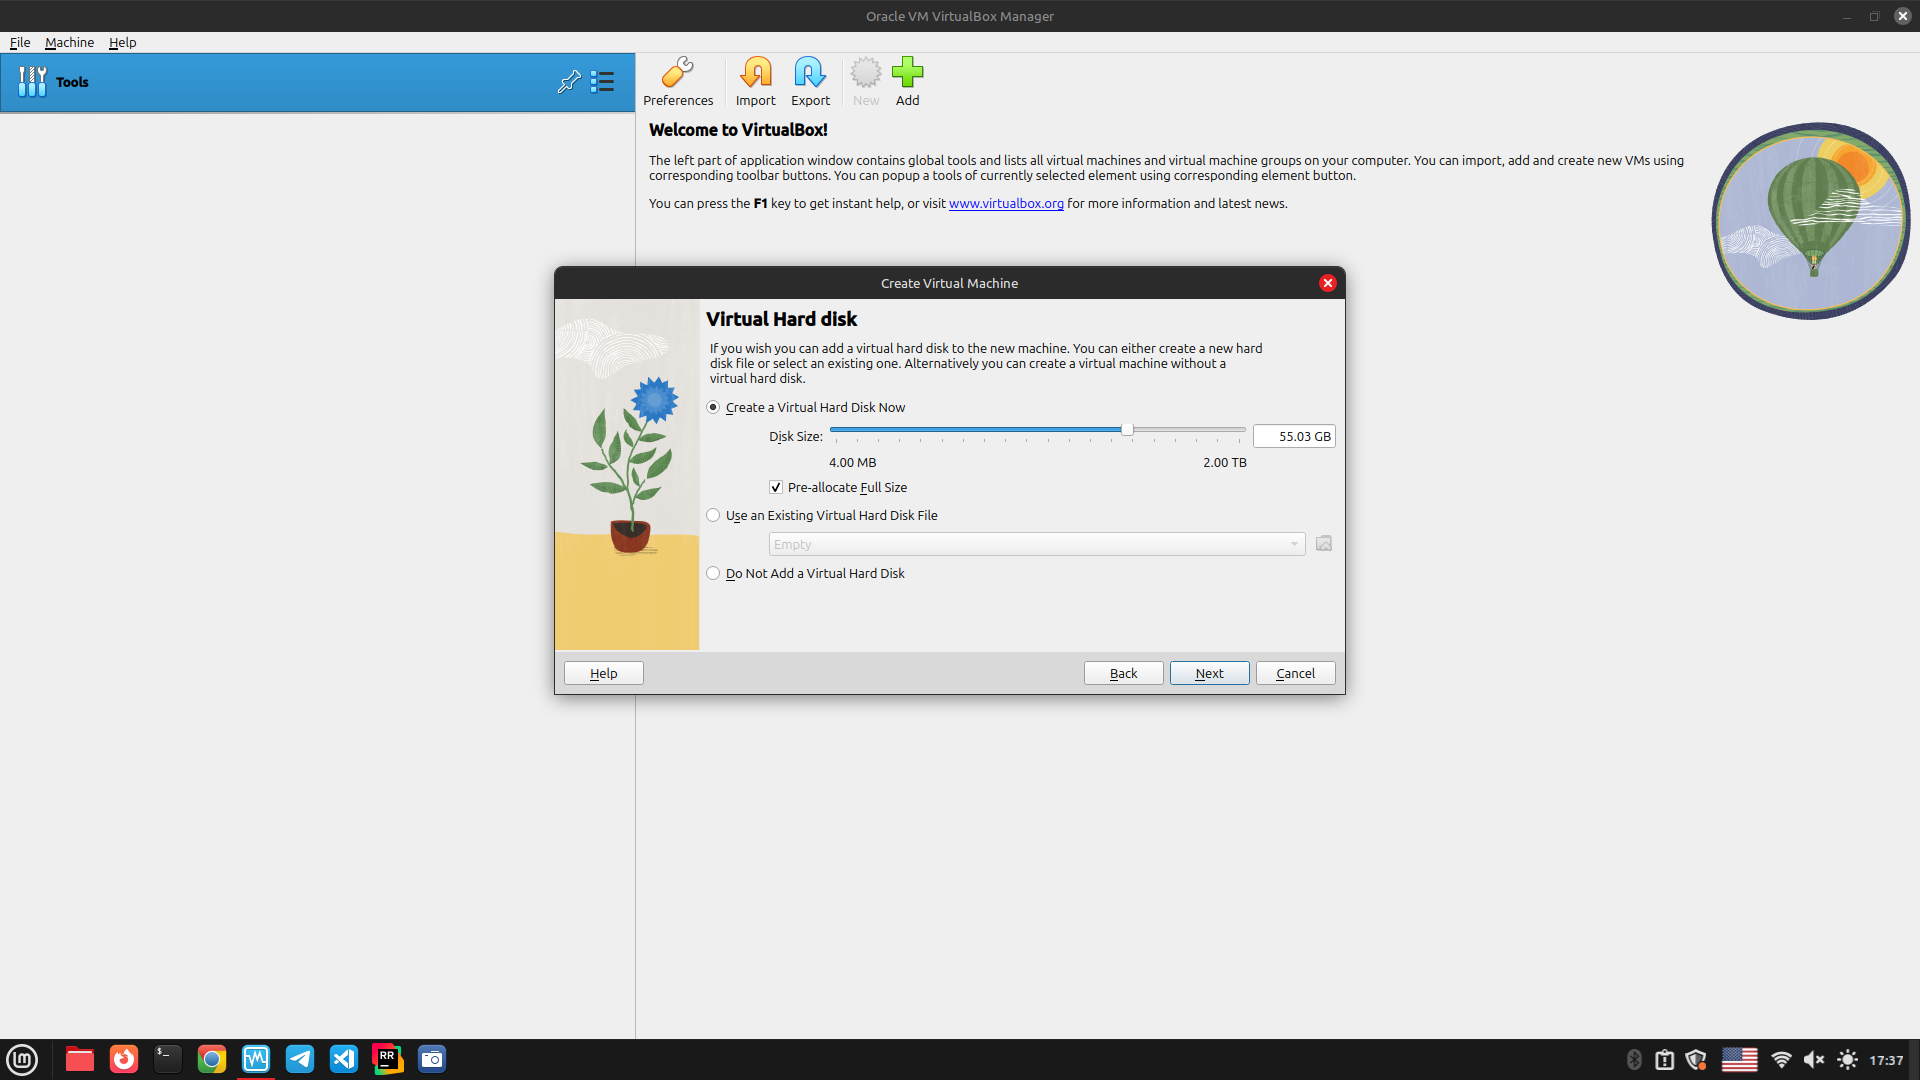
\includegraphics[width=0.8\textwidth]{report1-resources/3.png}
		\caption{ساخت دیسک مجازی و تعیین میزان حجم آن}
	\end{figure}

        \begin{figure}[H]
		\centering
		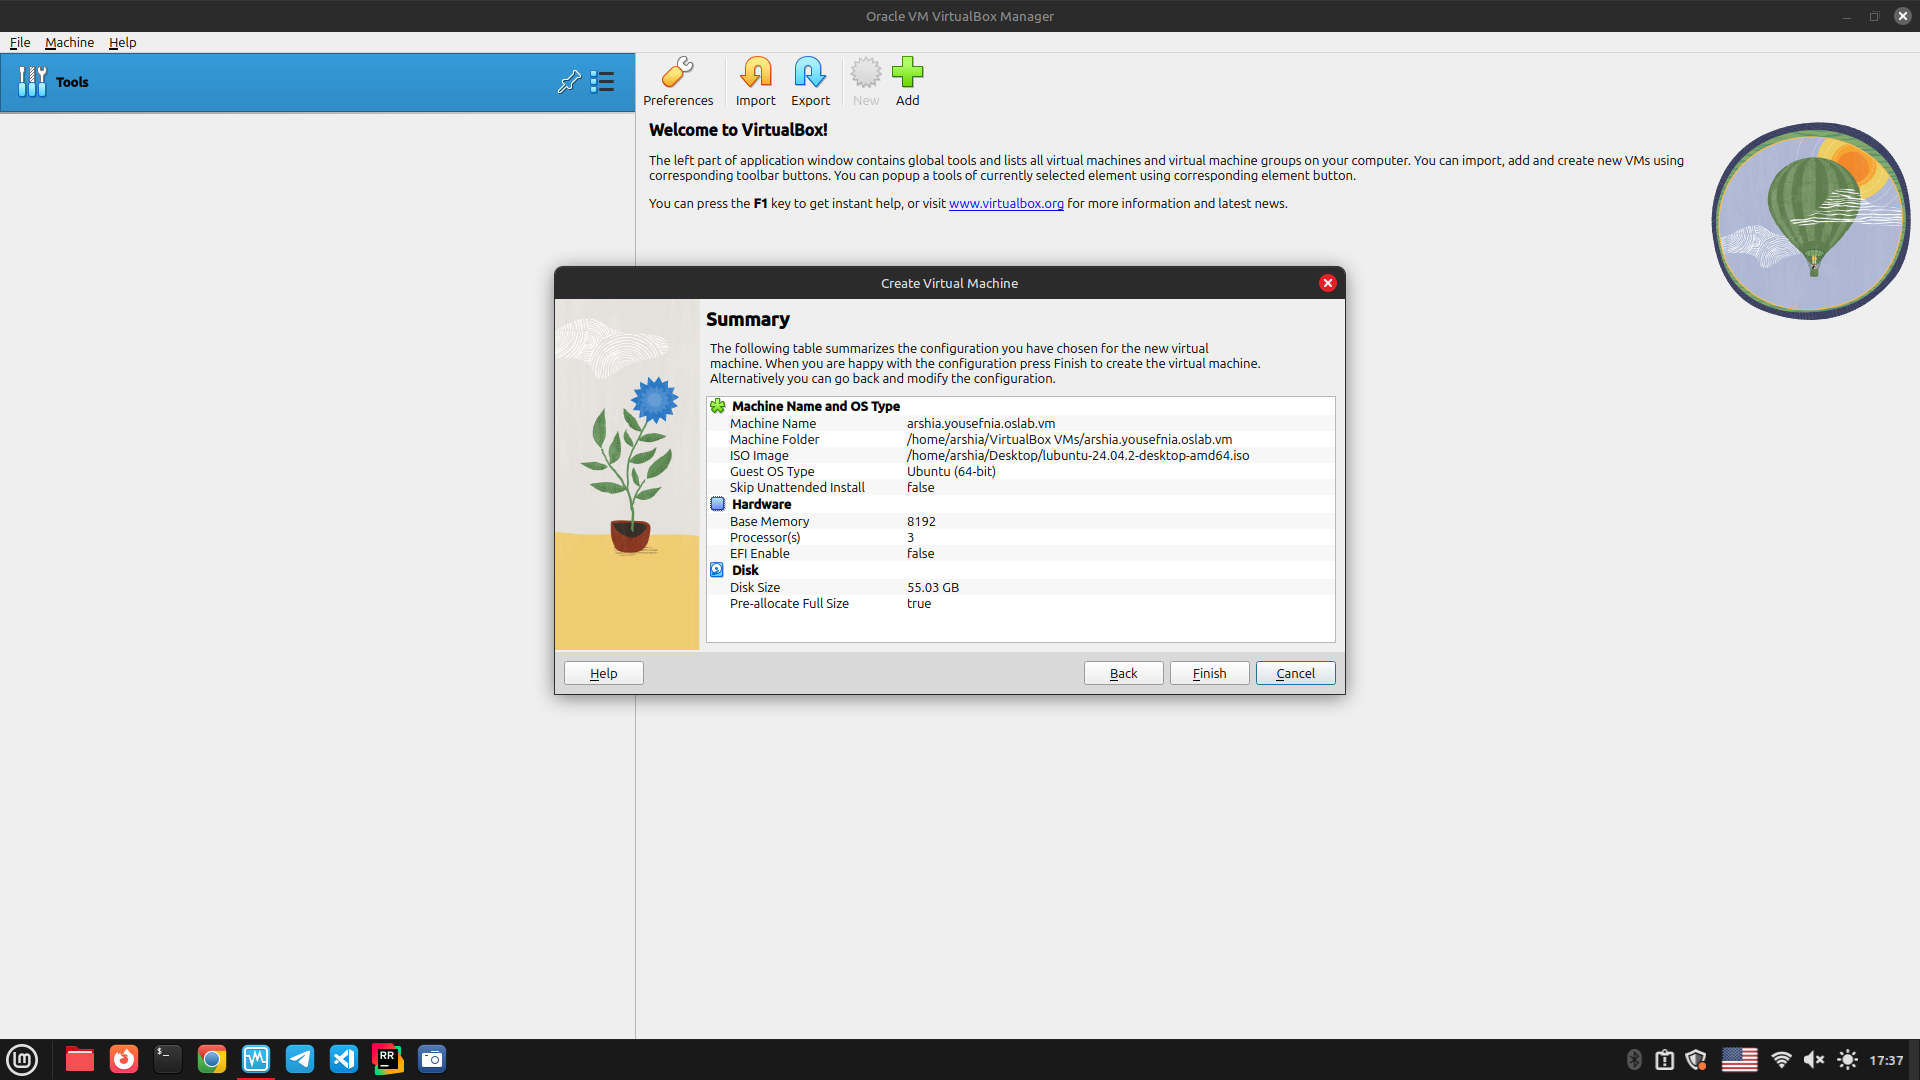
\includegraphics[width=0.8\textwidth]{report1-resources/4.png}
		\caption{خلاصه‌ی تنظیمات}
	\end{figure}

        \item 
        سپس مطابق خواسته‌ی صورت آزمایش، نسخه
        \textenglish{minimal}
        سیستم عامل را نصب می‌کنیم. هنگام اجرای ماشین مجازی، ابتدا به صفحه 
        \textenglish{boot}
        وارد می‌شویم. پس از انتخاب گزینه نصب سیستم عامل، باید در بخش
        \textenglish{customization}
        گزینه مینیمال را انتخاب کرده و سپس کاربر یا کاربرهای مورد نظر را ساخته و سیستم‌عامل را نصب می‌کنیم. در تصاویر زیر، مراحل آن را می‌توان مشاهده کرد.

        \begin{figure}[H]
		\centering
		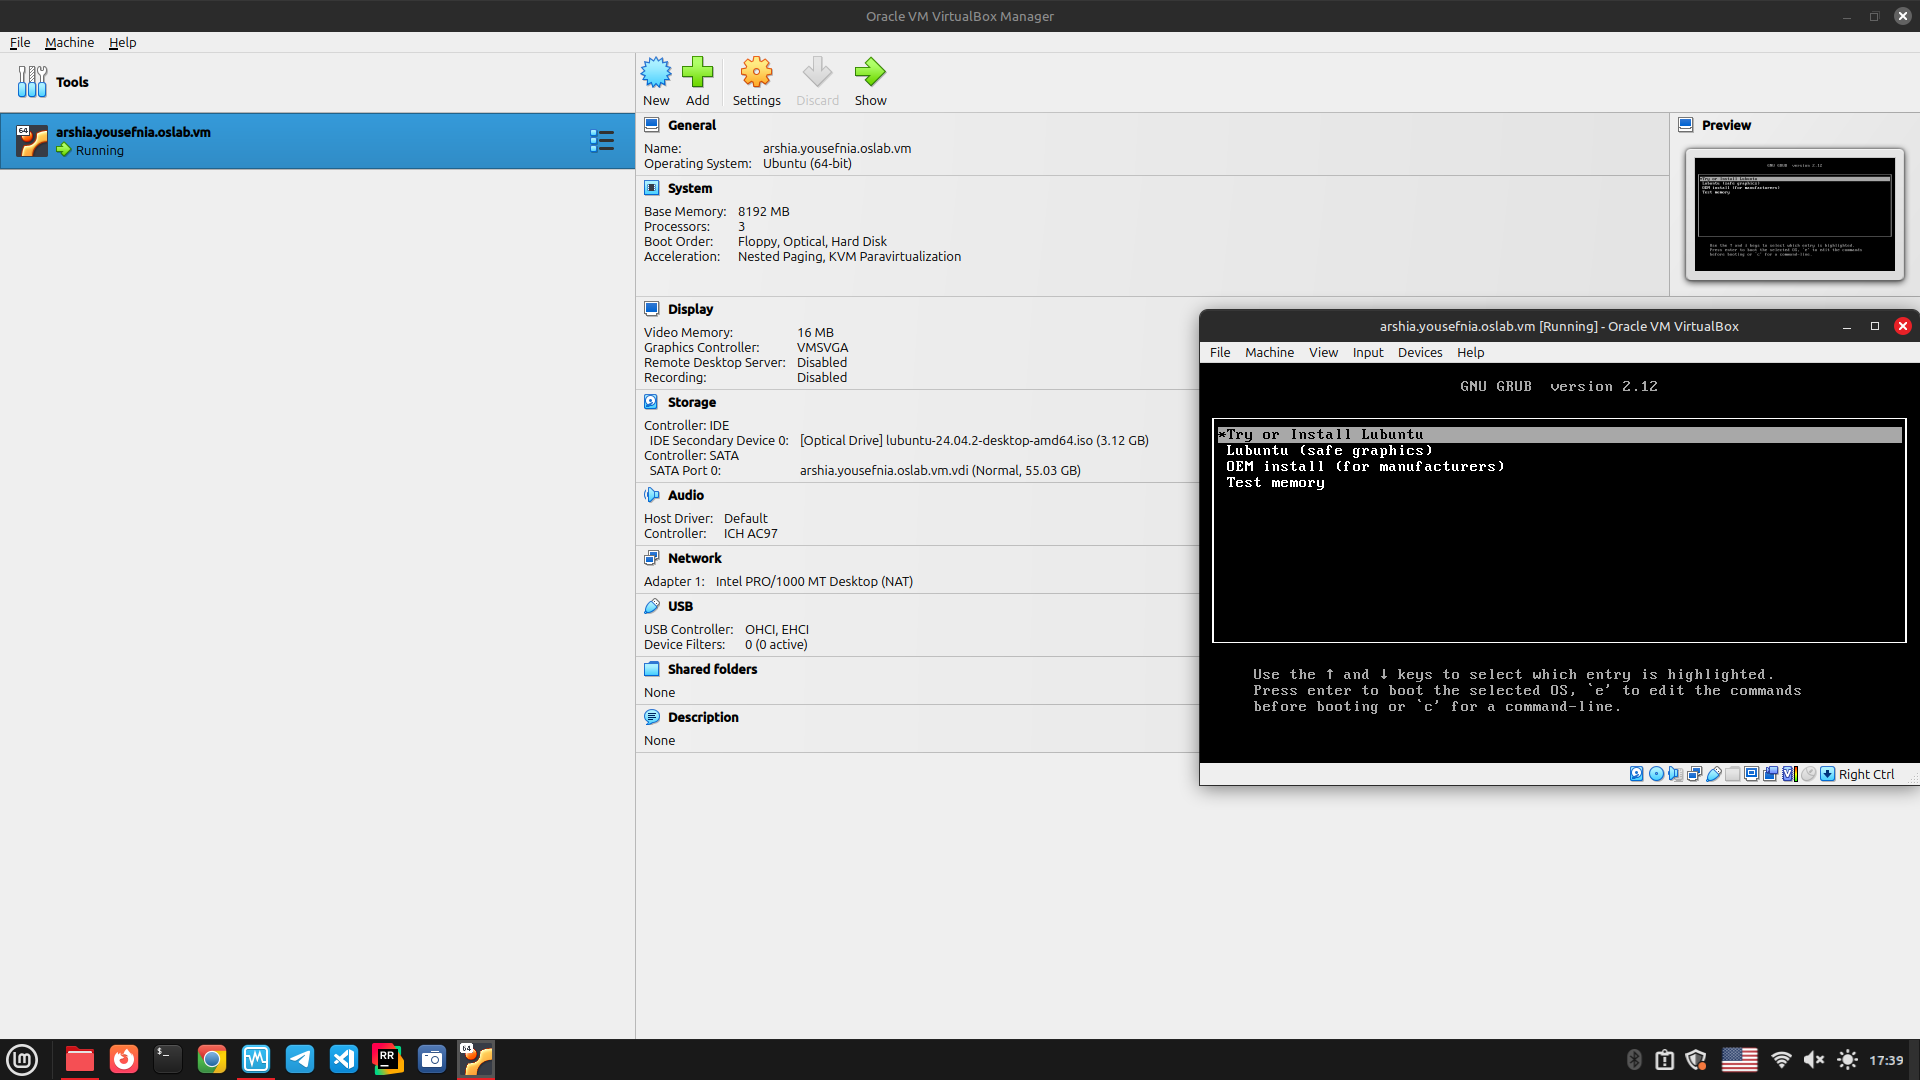
\includegraphics[width=0.8\textwidth]{report1-resources/5.png}
		\caption{صفحه \textenglish{boot}}
	\end{figure}

        \begin{figure}[H]
		\centering
		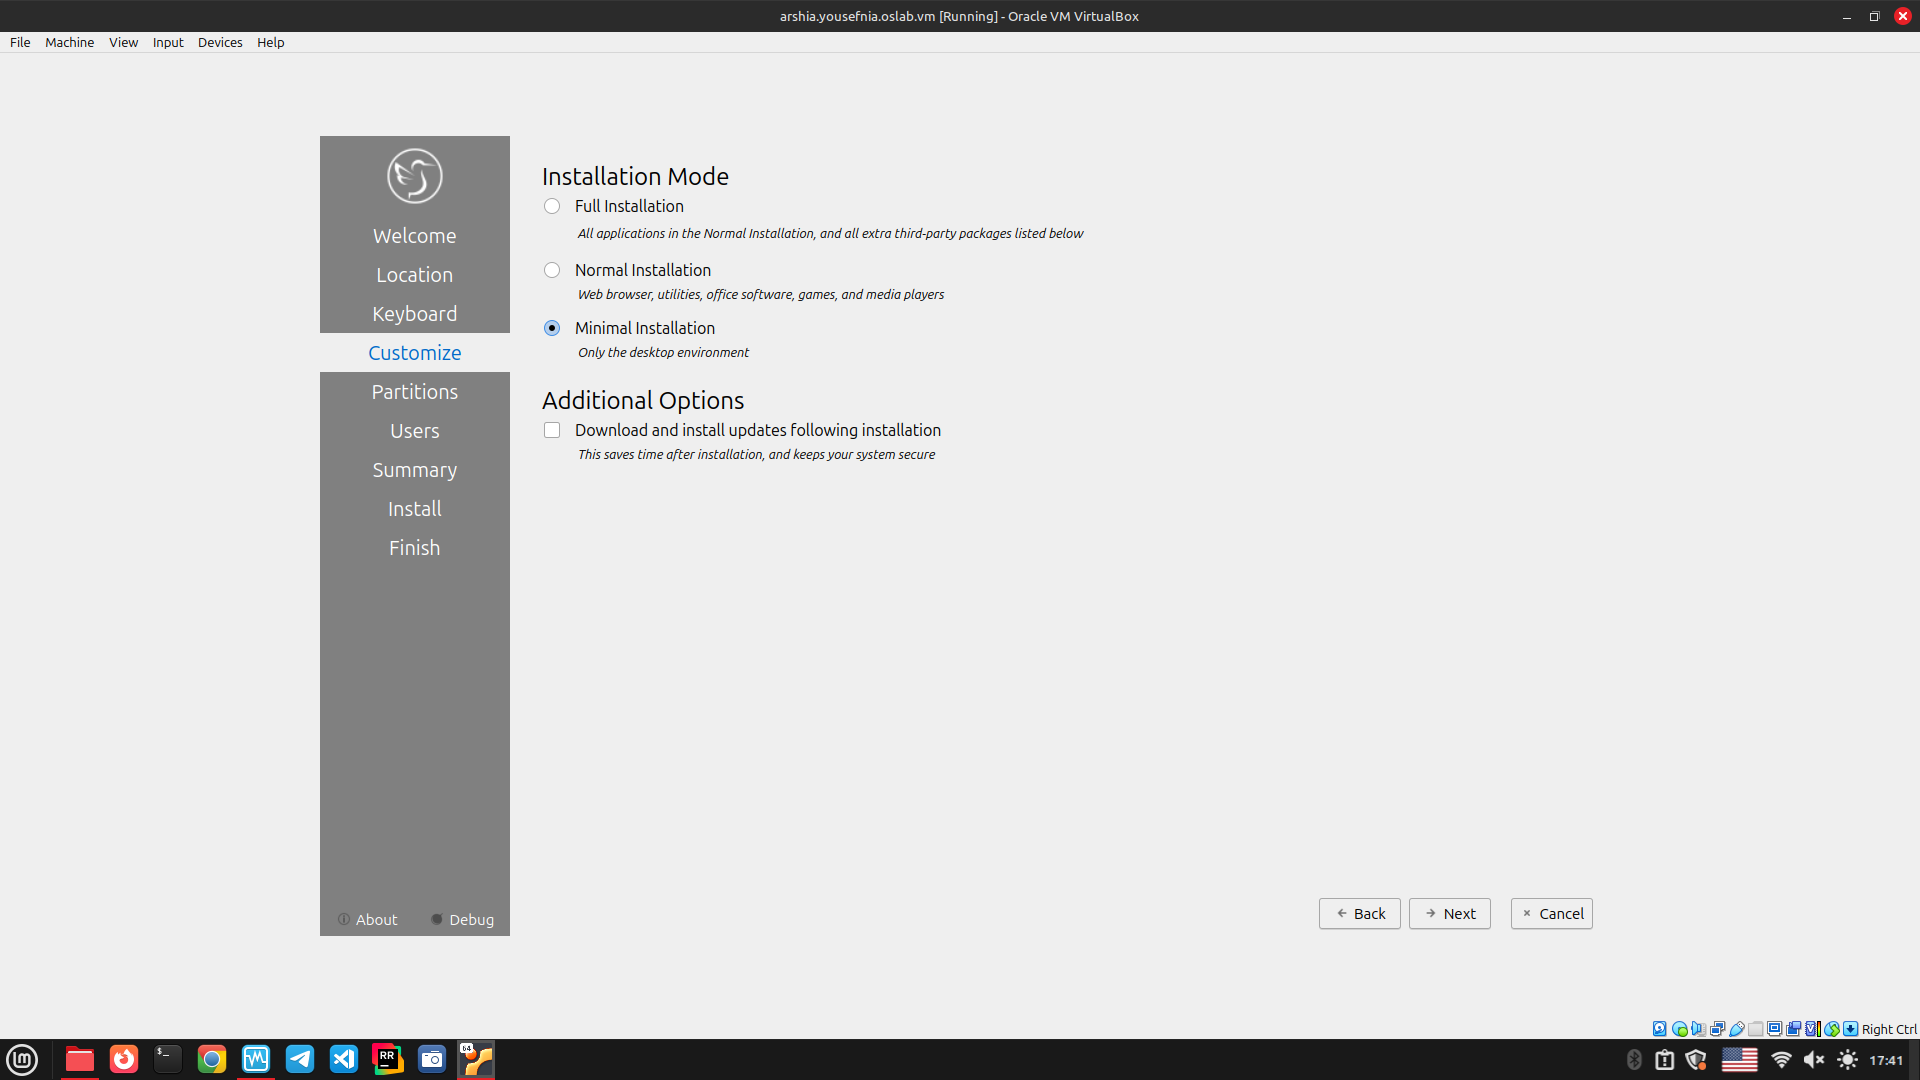
\includegraphics[width=0.8\textwidth]{report1-resources/6.png}
		\caption{انتخاب گزینه \textenglish{minimal}}
	\end{figure}

        \begin{figure}[H]
		\centering
		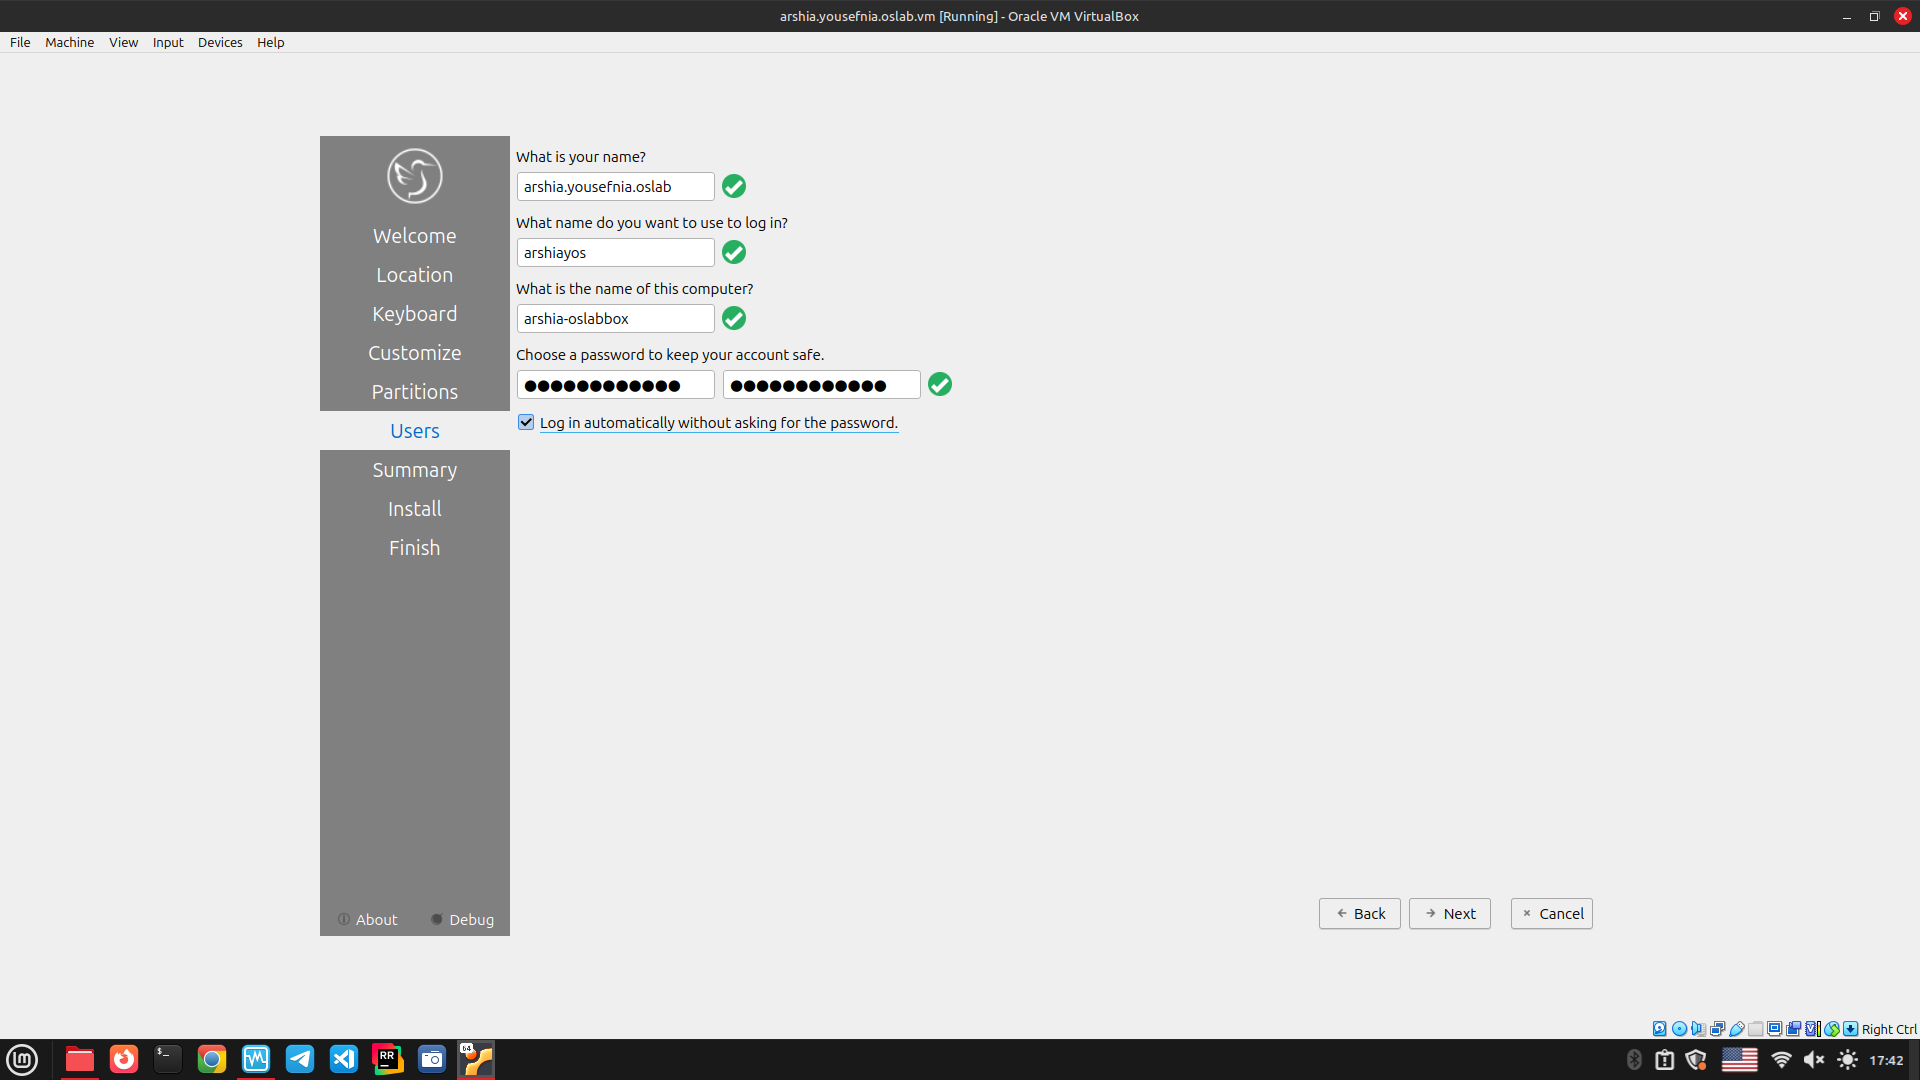
\includegraphics[width=0.8\textwidth]{report1-resources/7.png}
		\caption{وارد کردن مشخصات کاربر یا کاربرها}
	\end{figure}

        \begin{figure}[H]
		\centering
		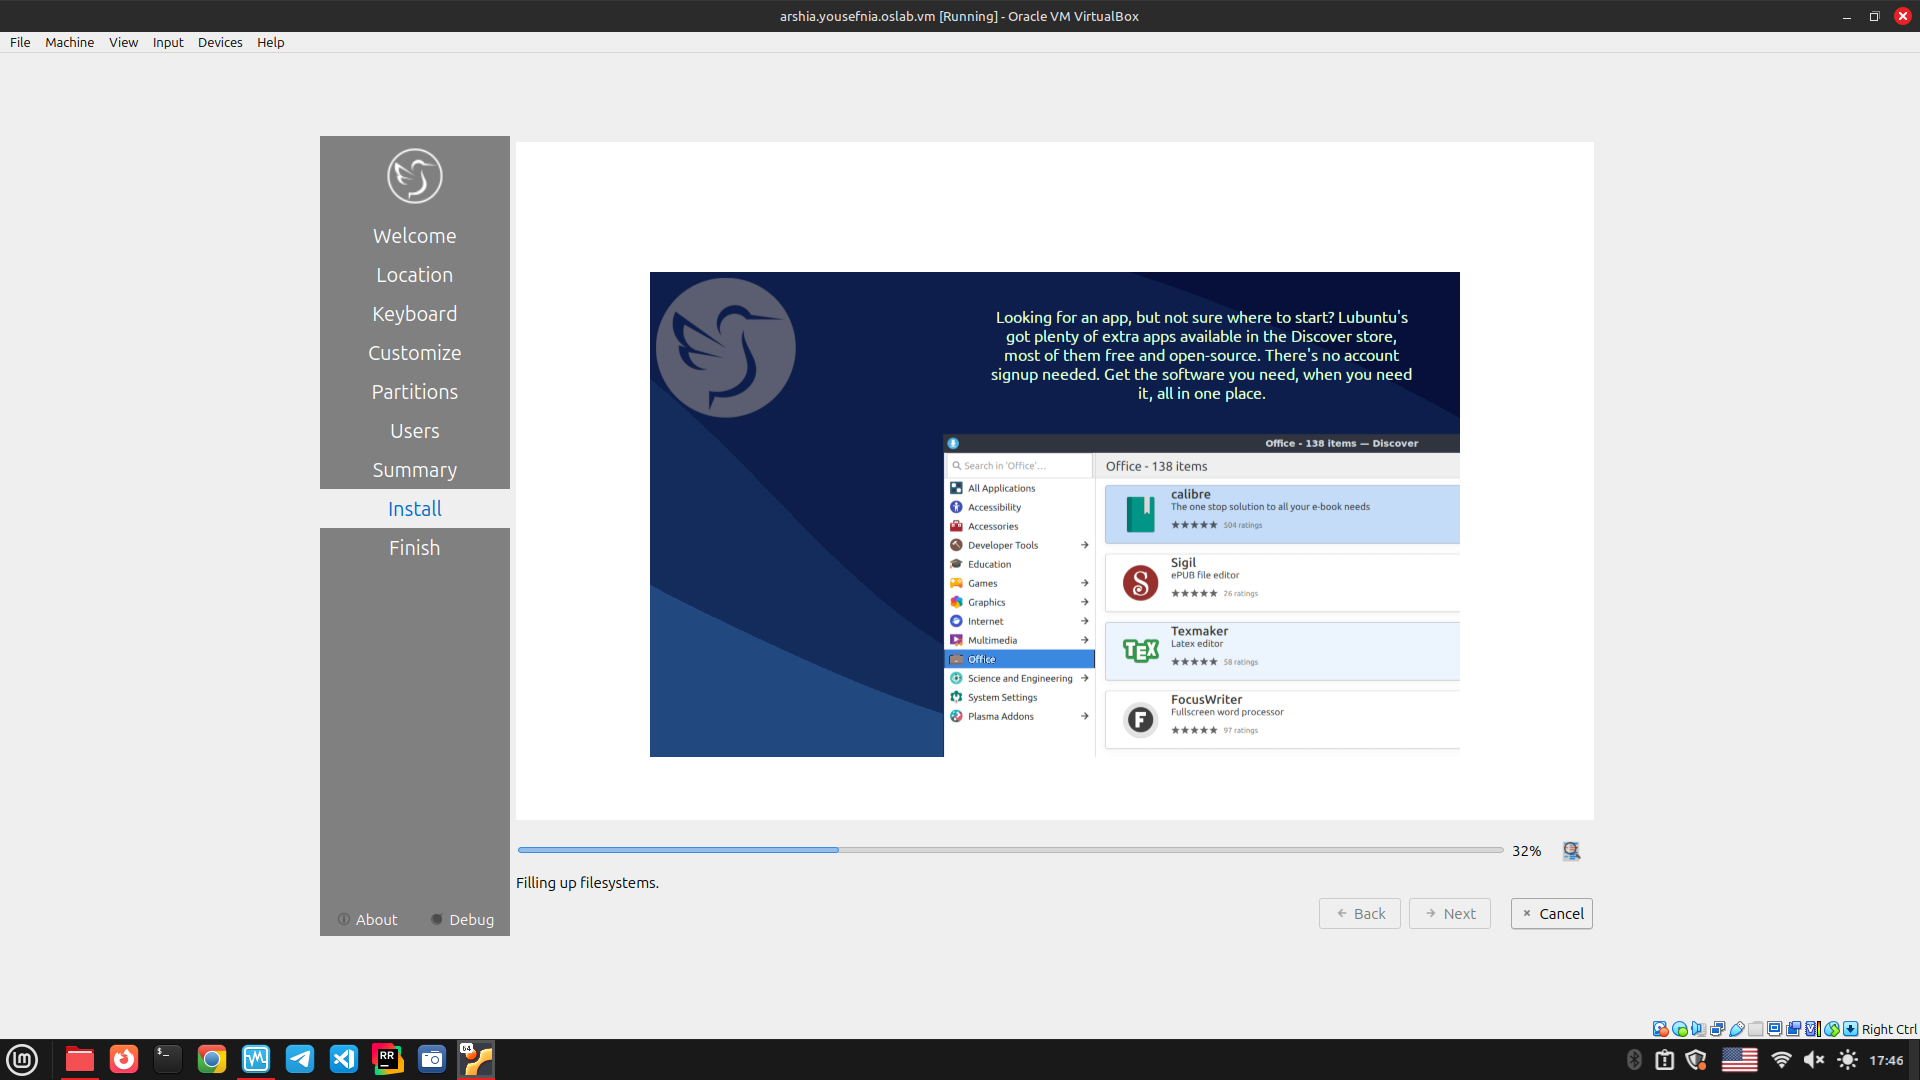
\includegraphics[width=0.8\textwidth]{report1-resources/8.png}
		\caption{نصب سیستم عامل}
	\end{figure}

        \end{enumerate}

        \subsection{آشنایی با دستورات پایه‌ی لینوکس}
        
        \begin{enumerate}
        \item با وارد کردن دستور 
        \textenglish{pwd}
        در ترمینال، آدرس دایرکتوری فعلی ترمینال چاپ می‌شود. در شکل
        \ref{im10}
        می‌توانید خروجی این دستور را مشاهده کنید.

        \item خروجی خواسته‌های این بخش نیز در شکل
        \ref{im10}
        قابل مشاهده است.

        \begin{figure}[H]
		\centering
		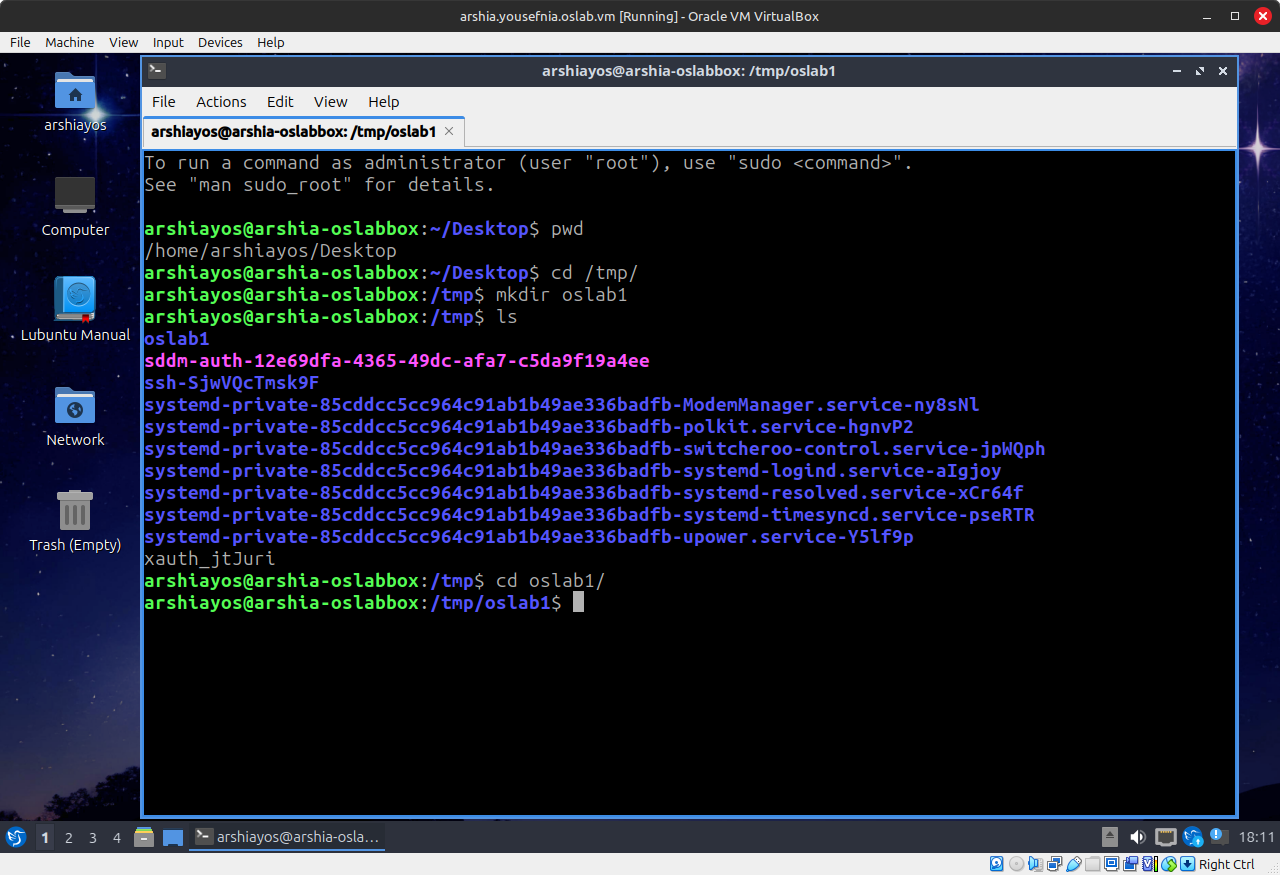
\includegraphics[width=0.8\textwidth]{report1-resources/10.png}
		\caption{دستورات \textenglish{pwd} و \textenglish{cd} و \textenglish{mkdir}}
            \label{im10}
	\end{figure}

        \item 
        ابتدا دستور
        \textenglish{nano information.txt}
        را می‌زنیم تا فایل خواسته شده ساخته شود. سپس نام و شماره دانشجویی را در آن وارد کرده و با اجرای
        \textenglish{ctrl+X}
        مانند شکل زیر برنامه از ما می‌پرسد که قصد ذخیره‌ی اطلاعات را داریم یا نه.
        
        \begin{figure}[H]
		\centering
		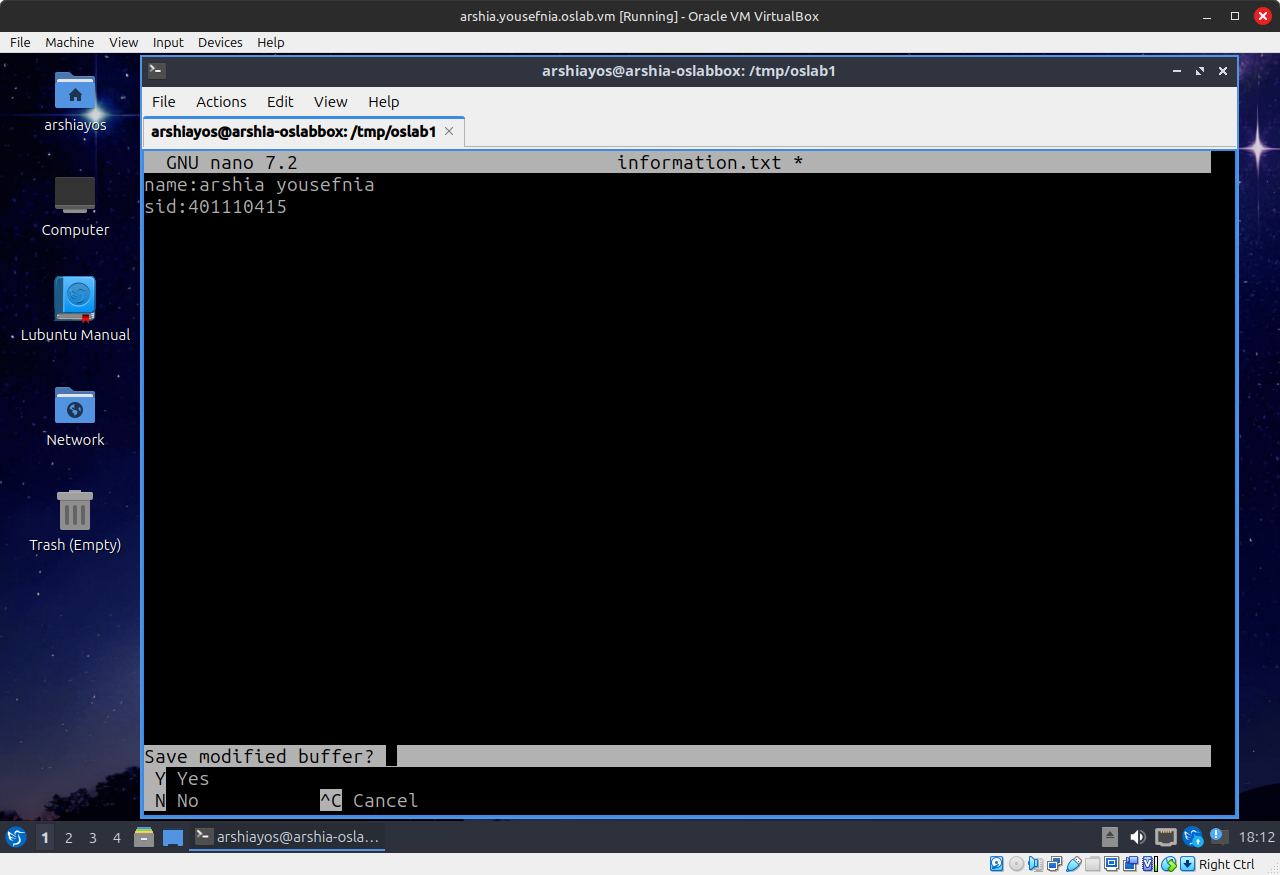
\includegraphics[width=0.8\textwidth]{report1-resources/11.png}
		\caption{محیط ادیتور \textenglish{nano}}
	\end{figure}

        \item 
        ابتدا با دستور
        cat
        نشان می‌دهیم که اطلاعات فایل بخش قبل به درستی ذخیره شده است. سپس با دستور 
        mv
        آن فایل را کات کرده و با نام
        myinformation.txt
        آن را در همان دایرکتوری قرار می‌دهیم. به این صورت می‌توانیم نام فایل‌ها را تغییر دهیم.

        \begin{figure}[H]
		\centering
		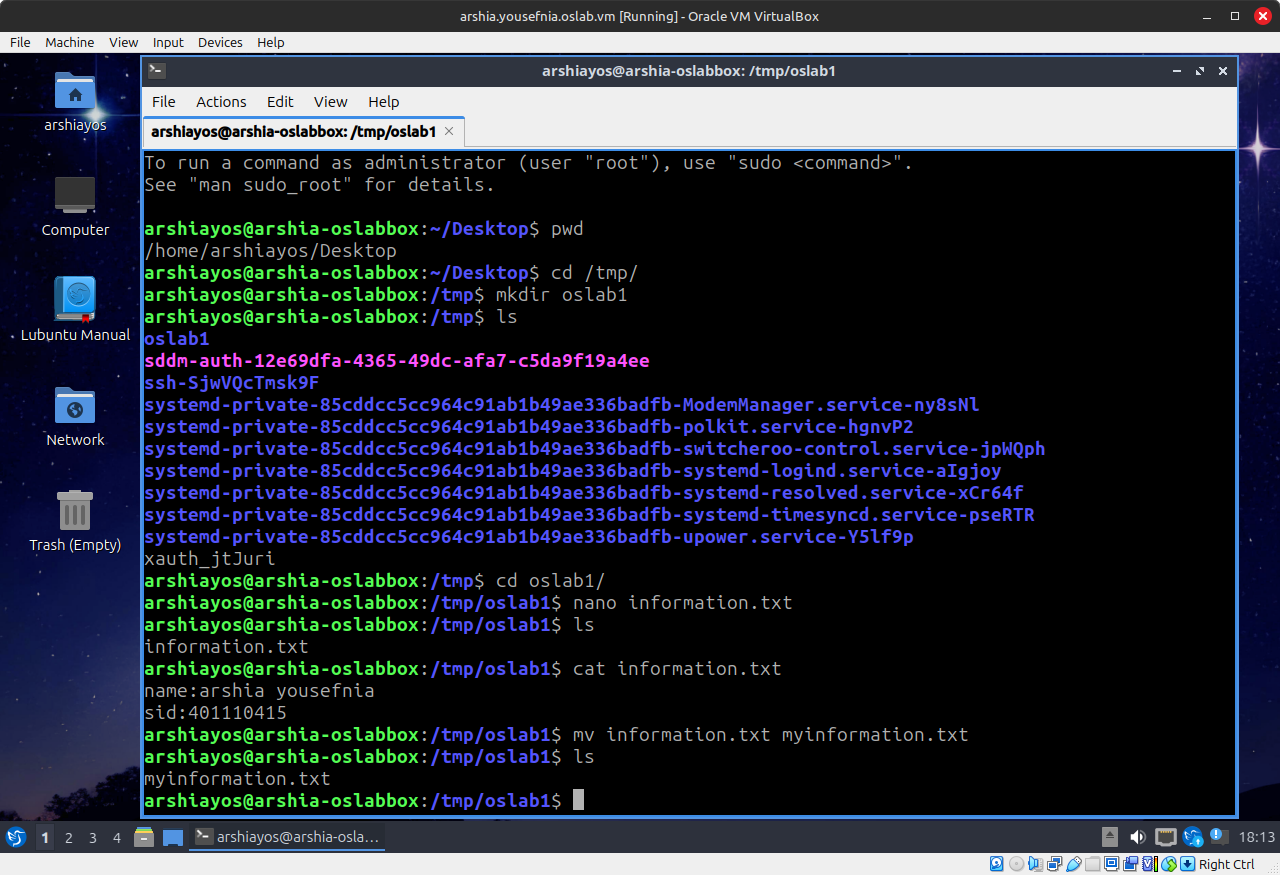
\includegraphics[width=0.8\textwidth]{report1-resources/12.png}
		\caption{تغییر نام فایل با دستور mv}
	\end{figure}

        \item 
        با دستور 
        cp
        و با فرمت
        
        \begin{english}
            cp <src-address> <dst-address>
        \end{english}
        
        می‌توانیم از فایل‌ها کپی بگیریم.

        \begin{figure}[H]
		\centering
		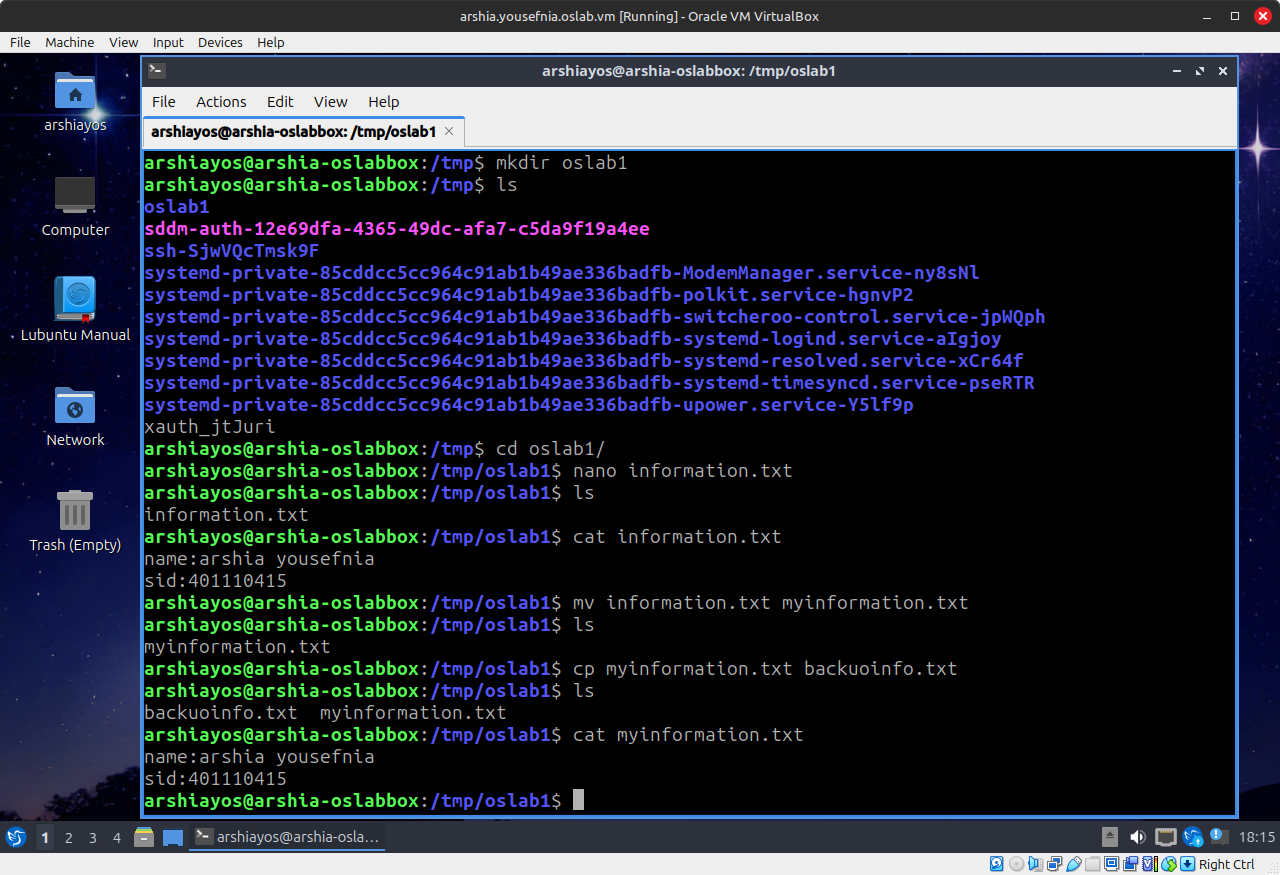
\includegraphics[width=0.8\textwidth]{report1-resources/13.png}
		\caption{کپی گرفتن از فایل}
            \label{im13}
	\end{figure}

        \item 
        همانطور که از شکل
        \ref{im13}
        می‌توان مشاهده کرد، محتویات فایل کپی شده و فایل اصلی یکسان است.

        \item 
        در تصویر زیر، می‌توان دو دستور گفته شده را مشاهده کرده و خروجی آنها را دید. همانطور که از تصویر قابل مشاهده است، استفاده از عملگر
        \textenglish{>}
        خروجی دستور سمت چپش را در فایل سمت راست می‌ریزد، و طی آن محتویات قبلی آن فایل از بین می‌رود. اما استفاده از عملگر
        \textenglish{>>}
        محتویات خروجی دستور را به آن فایل
        \textenglish{append}
        می‌کند. یعنی آن را به انتهای محتویات آن فایل اضافه می‌کند.

        \begin{figure}[H]
		\centering
		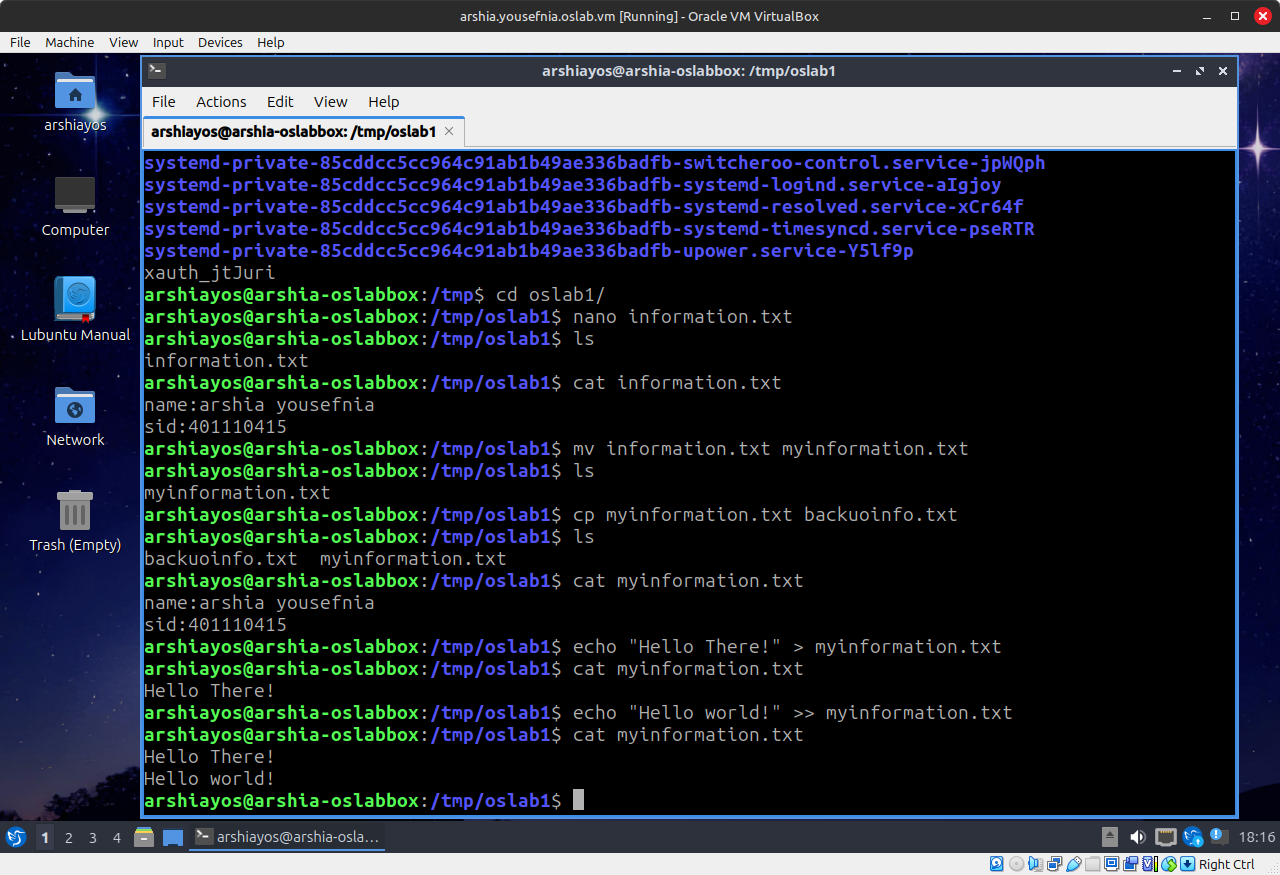
\includegraphics[width=0.8\textwidth]{report1-resources/14.png}
		\caption{بررسی عملگرهای \textenglish{>} و \textenglish{>>}}
	\end{figure}

        \item 
        می‌توان با دستور 
        cat
        و با کمک عملگر 
        \textenglish{>}،
        بدون استفاده از ادیتور، فایل جدید با محتوای دلخواه (یا فایل قدیم با محتوای جدید) ساخت.
        وقتی دستور را به فرمت

        \begin{english}
            cat > <filename>
        \end{english}

        وارد می‌کنیم، می‌توان هر محتوایی که خواستیم بنویسیم و تا وقتی که  از
        \textenglish{ctrl+C}
        استفاده نکرده‌ایم، هر چیزی که در ترمینال می‌نویسیم (حتی 
        \textenglish{\textbackslash{}n})
        در فایل قرار می‌گیرد.

        \begin{figure}[H]
		\centering
		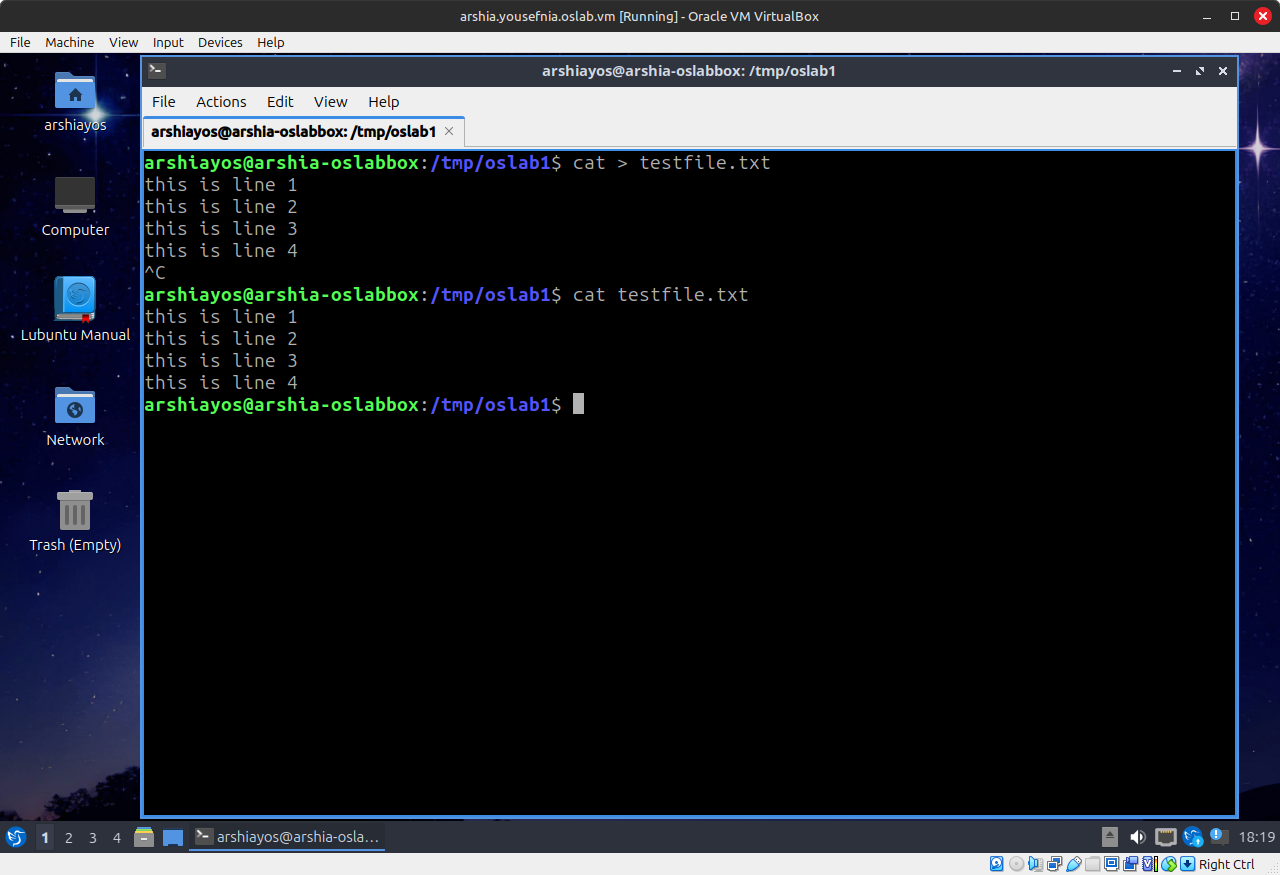
\includegraphics[width=0.8\textwidth]{report1-resources/15.png}
		\caption{نوشتن در فایل با کمک دستور cat}
	\end{figure}

        \item 
        با اجرای دستور
        \textenglish{ps aux}
        می‌توانیم لیست کل پردازه‌های در حال اجرا را مشاهده کنیم. در شکل‌های
        \ref{im16}
        تا
        \ref{im19}
        می‌توان این پردازه‌ها را دید.

        \begin{figure}[H]
		\centering
		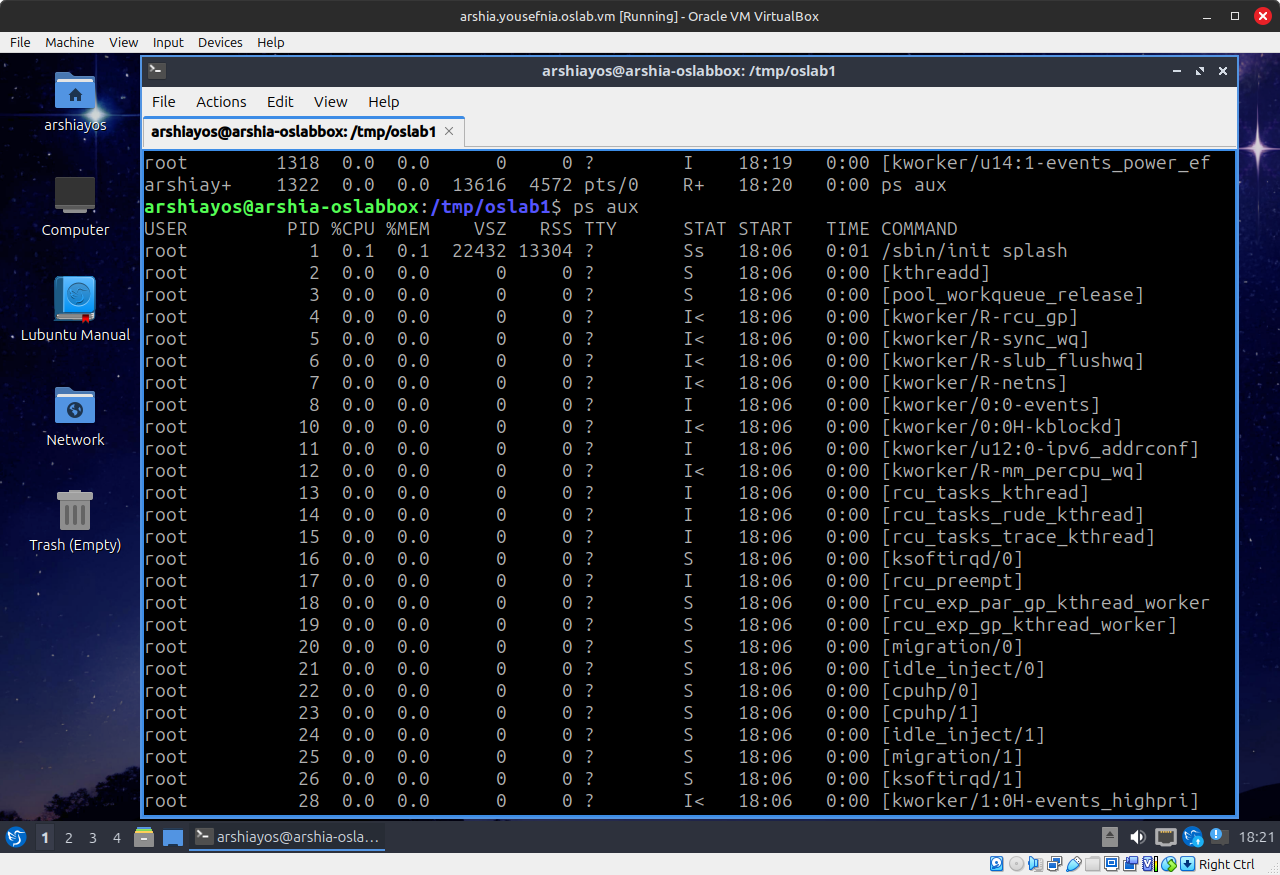
\includegraphics[width=0.8\textwidth]{report1-resources/16.png}
		\caption{لیست پردازه‌های درحال اجرا (بخش اول)}
            \label{im16}
	\end{figure}

        \begin{figure}[H]
		\centering
		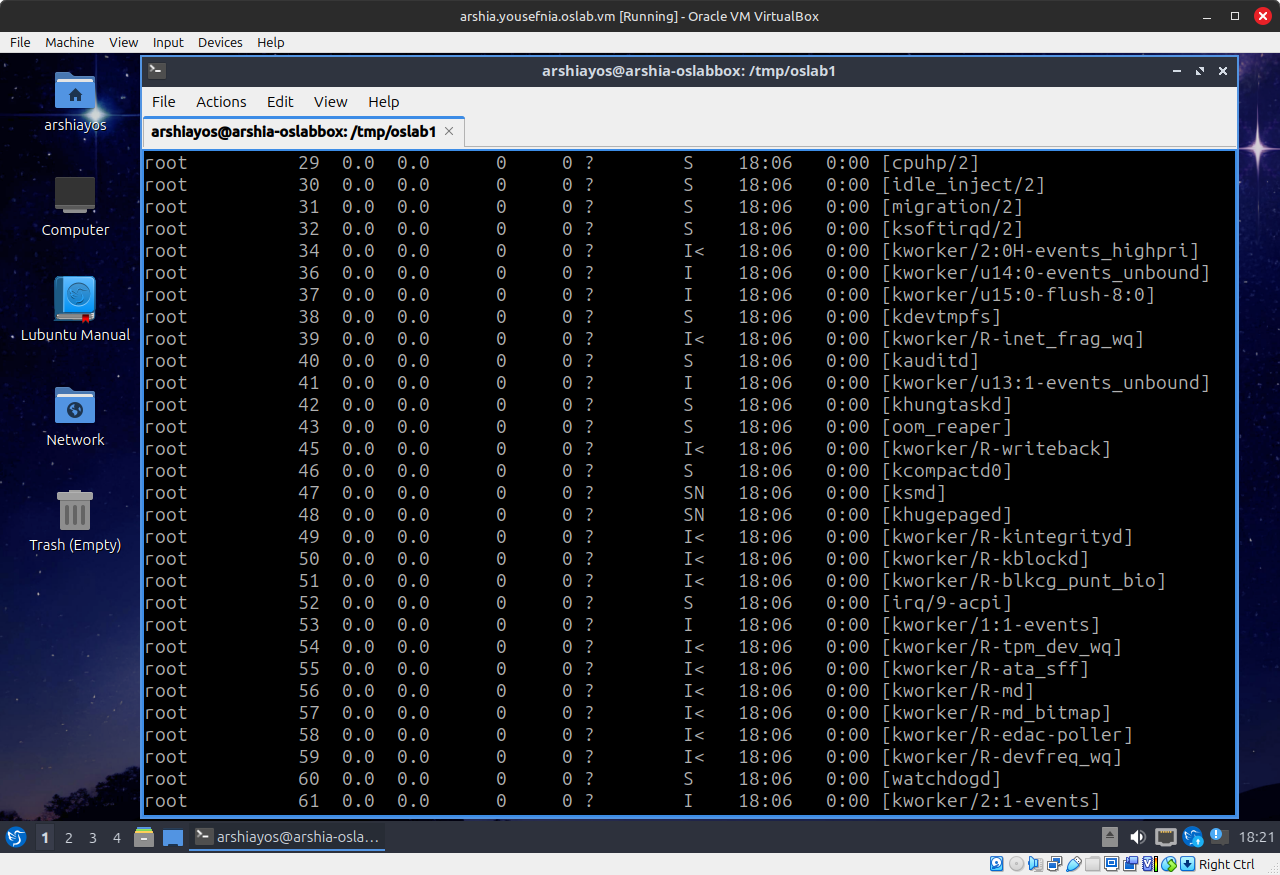
\includegraphics[width=0.8\textwidth]{report1-resources/17.png}
		\caption{لیست پردازه‌های درحال اجرا (بخش دوم)}
	\end{figure}

        \begin{figure}[H]
		\centering
		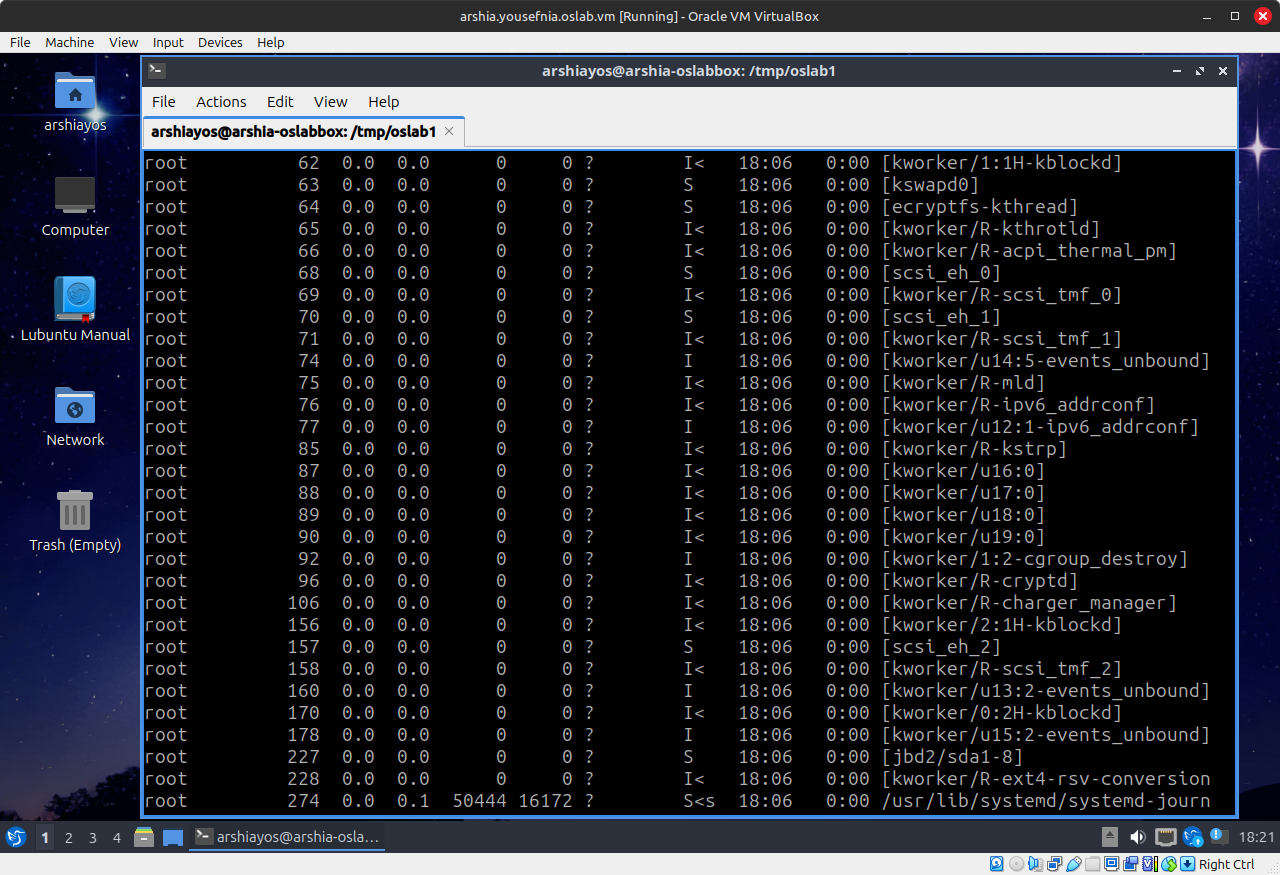
\includegraphics[width=0.8\textwidth]{report1-resources/18.png}
		\caption{لیست پردازه‌های درحال اجرا (بخش سوم)}
	\end{figure}

        \begin{figure}[H]
		\centering
		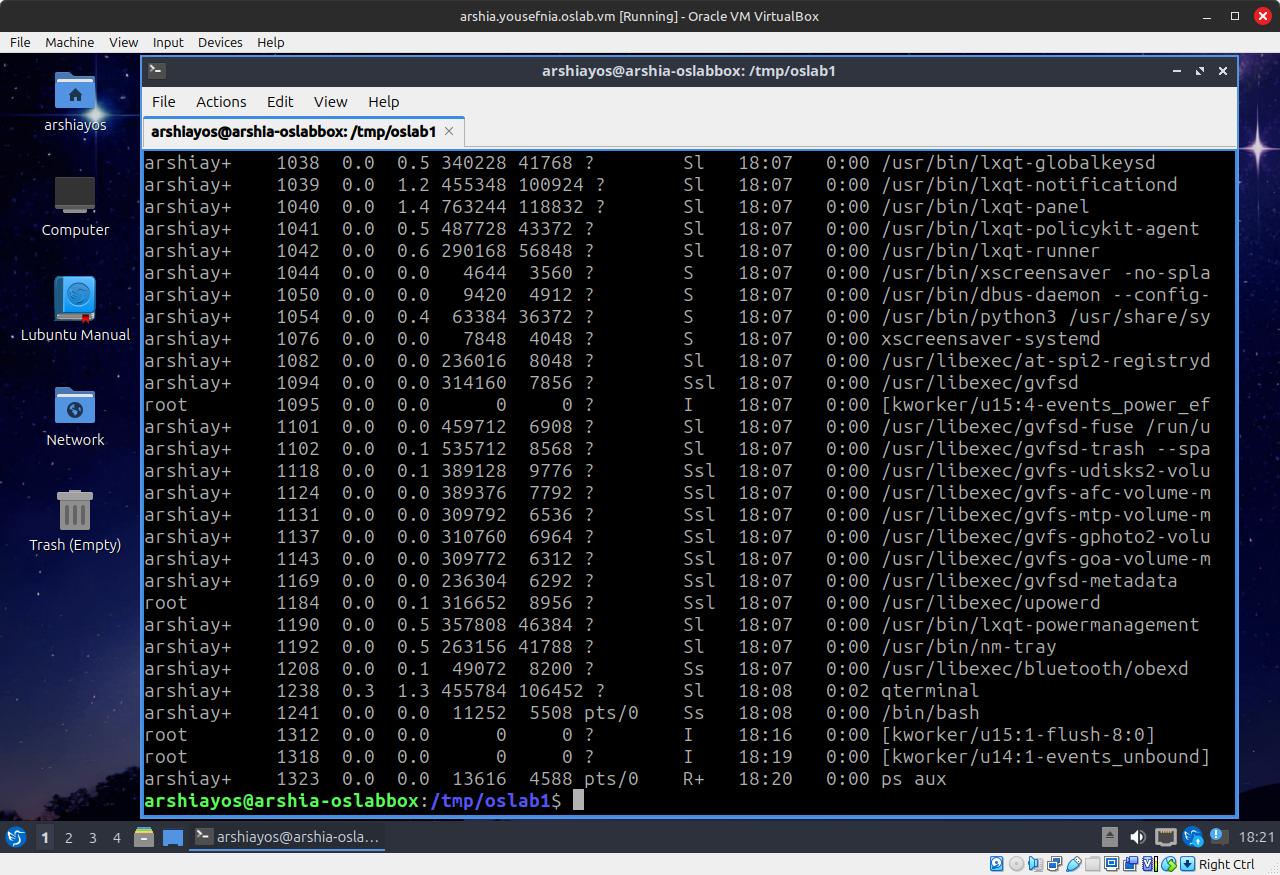
\includegraphics[width=0.8\textwidth]{report1-resources/19.png}
		\caption{لیست پردازه‌های درحال اجرا (بخش آخر)}
            \label{im19}
	\end{figure}

        \item 
        با دستور
        \textenglish{ps}
        و استفاده از آپشن 
        \textenglish{-e}
        می‌توان تمام پردازه‌ها را مشاهده کرد. همچنین با آپشن
        \textenglish{-o}
        می‌توان نام ستون‌هایی که می‌خواهیم در خروجی بیایند را مشخص کرد. برای مثال 
        comm
        برای نام پردازه به کار می‌رود (به طور دقیق‌تر نام دستوری که مربوط به آن پردازه است).

        بنابراین با دستور
        \textenglish{ps -eo comm}
        می‌توان نام تمام پردازه‌ها را اجرا کرد. همچنین با استفاده از عملگر 
        \textenglish{|}
        که خروجی دستور سمت چپ را به عنوان ورودی به دستور سمت راست می‌دهد، می‌توان روی لیست تمام پردازه‌ها، دستور 
        grep
        را اجرا کرد و با کمک
        \textenglish{grep "a"}
        می‌توان نام تمام پردازه‌هایی که در آنها حرف 
        a
        وجود دارد را مشاهده کرد. در شکل‌
        \ref{im20}
        فقط نام آن پردازه‌ها طبق توضیحات گفته شده آورده شده است، و در شکل
        \ref{im21}
        کلیه‌ی اطلاعات آورده شده‌اند.

        \begin{figure}[H]
		\centering
		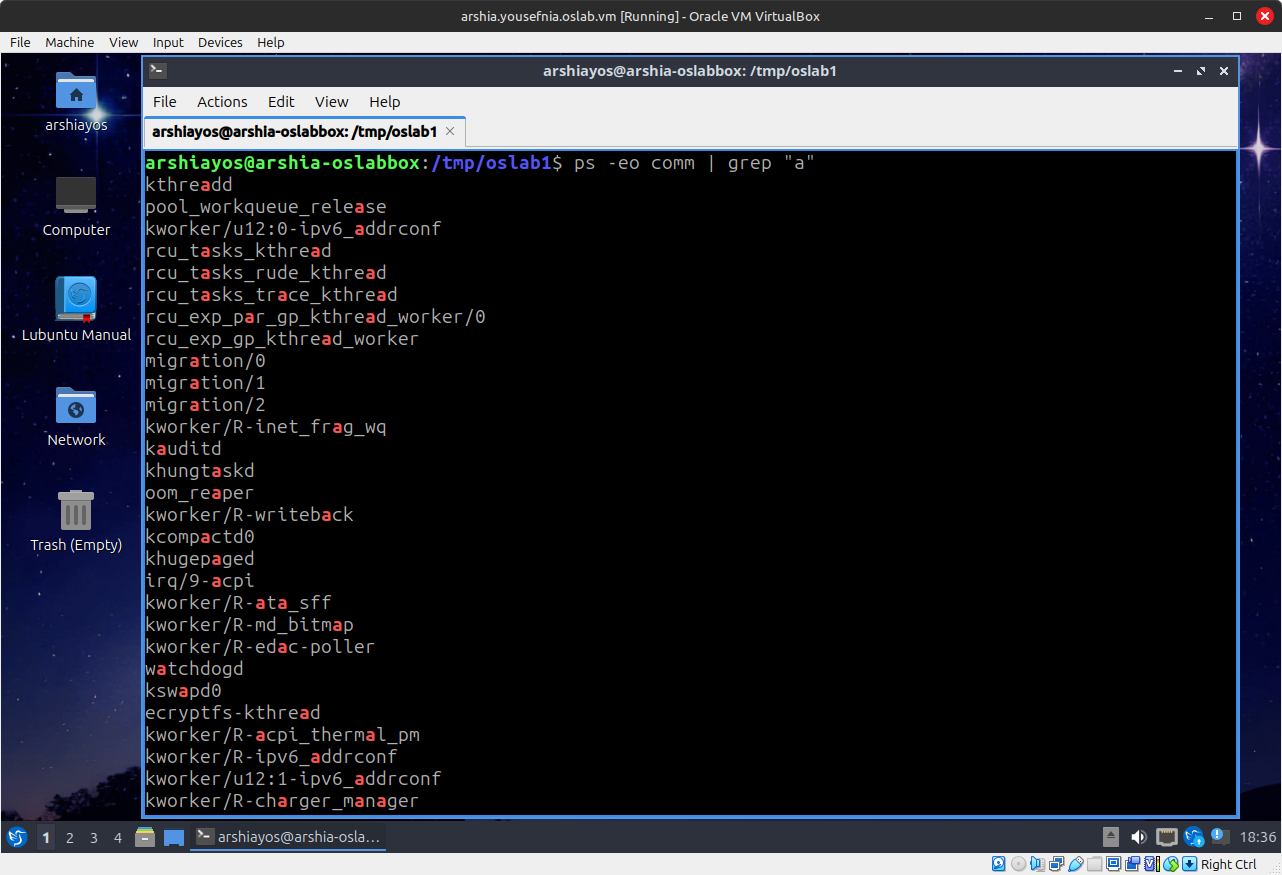
\includegraphics[width=0.8\textwidth]{report1-resources/20.png}
		\caption{نام پردازه‌هایی که در نامشان حرف a وجود دارد}
            \label{im20}
	\end{figure}

        \begin{figure}[H]
		\centering
		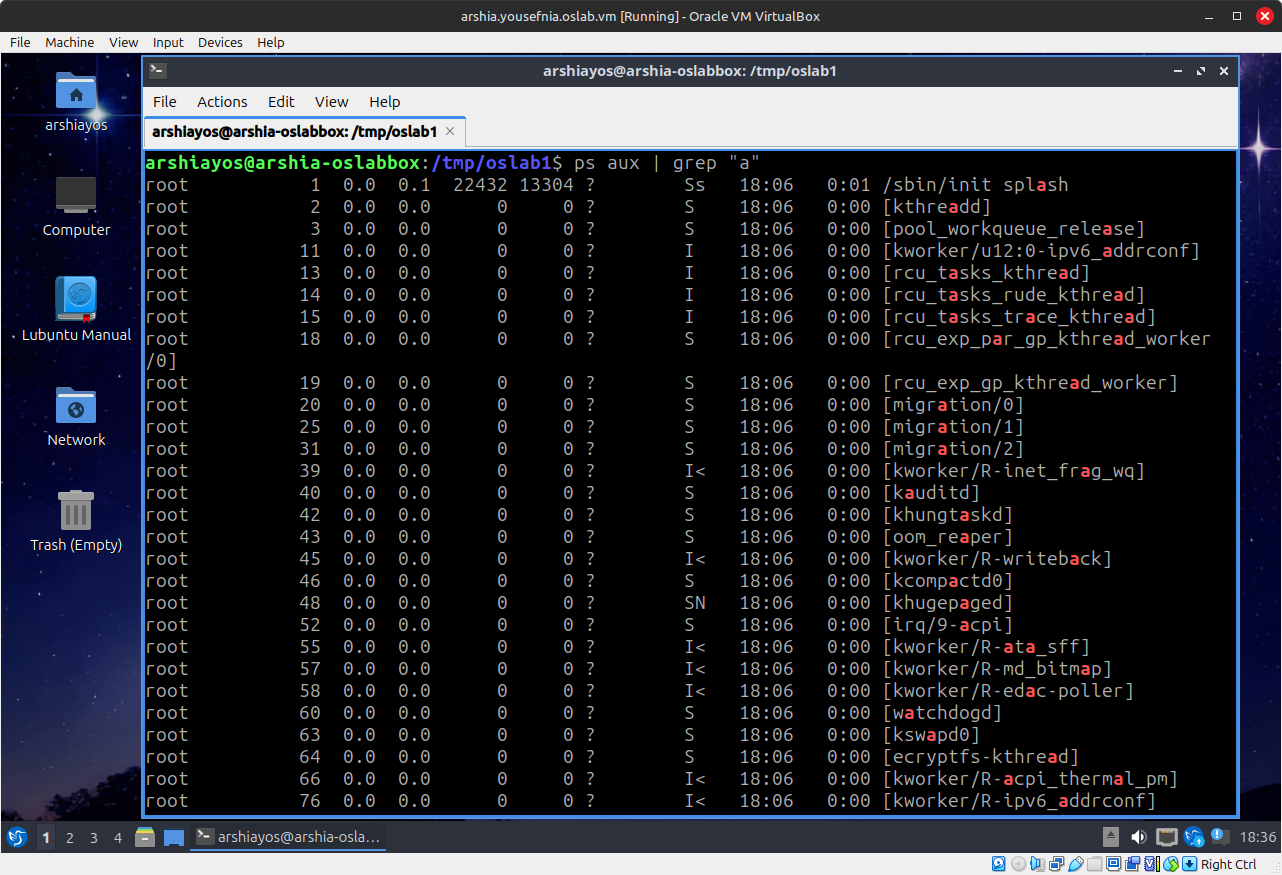
\includegraphics[width=0.8\textwidth]{report1-resources/21.png}
		\caption{کلیه‌ی اطلاعات پردازه‌هایی که در آنها حرف a وجود دارد}
            \label{im21}
	\end{figure}

        \item خروجی دستور 
        ls
        در این بخش را در شکل زیر می‌توانید مشاهده کنید.

        \begin{figure}[H]
		\centering
		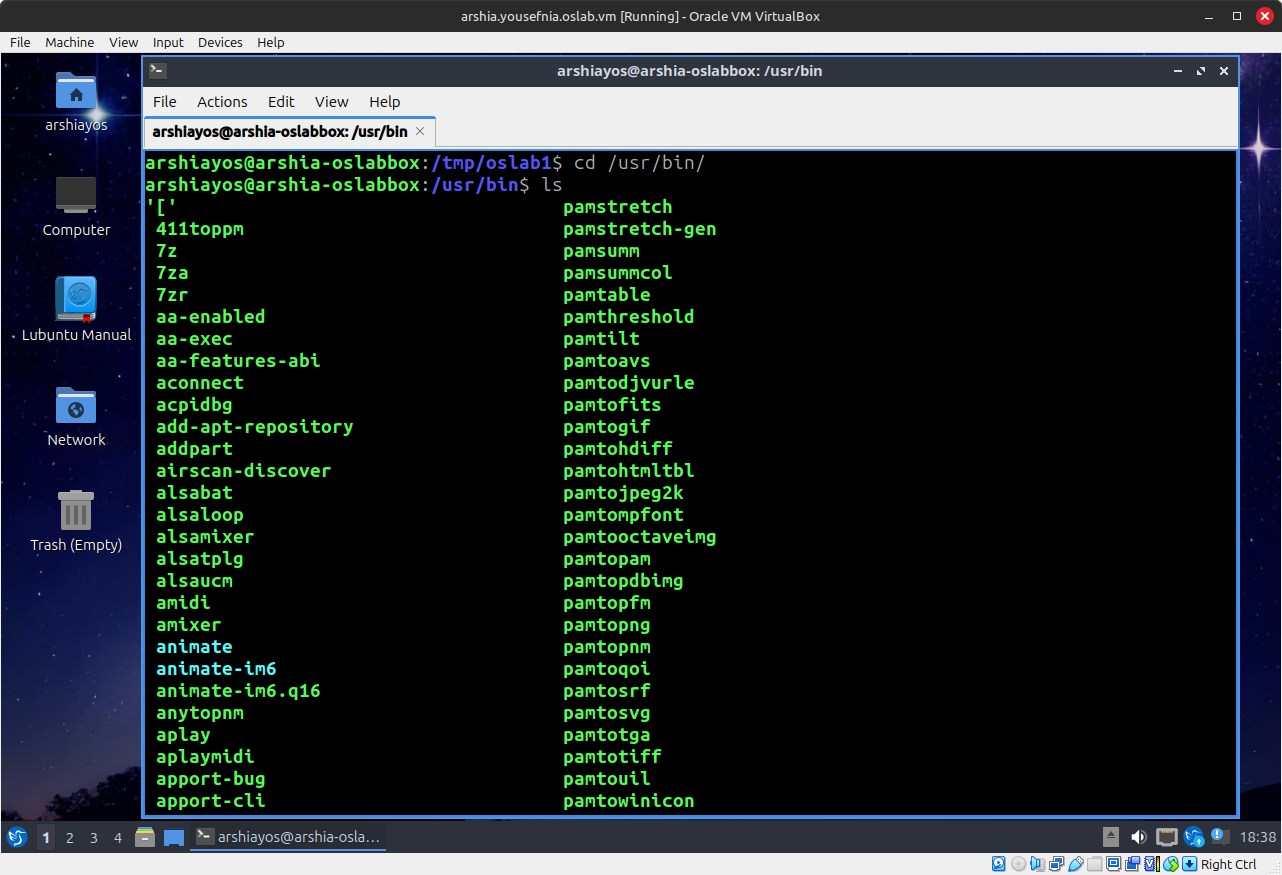
\includegraphics[width=0.8\textwidth]{report1-resources/22.png}
		\caption{بخشی از محتویات دایرکتوری \textenglish{/usr/bin/}}
	\end{figure}

        \item
        آپشن 
        \textenglish{-l}
        اطلاعات اضافه‌تر درمورد فایل‌ها مانند مالک فایل، سطوح دسترسی فایل، حجم فایل و ... را نشان می‌دهد. همچنین آپشن
        \textenglish{-h}
        حجم فایل‌ها را به فرمتی قابل فهم‌تر (برای مثال برحسب کیلوبایت یا مگابایت) بیان می‌کند.

        همچنین با دستور
        head
        برای اینکه صفحه شلوغ نشود، فقط 20 فایل اول را نشان می‌دهیم.

        \begin{figure}[H]
		\centering
		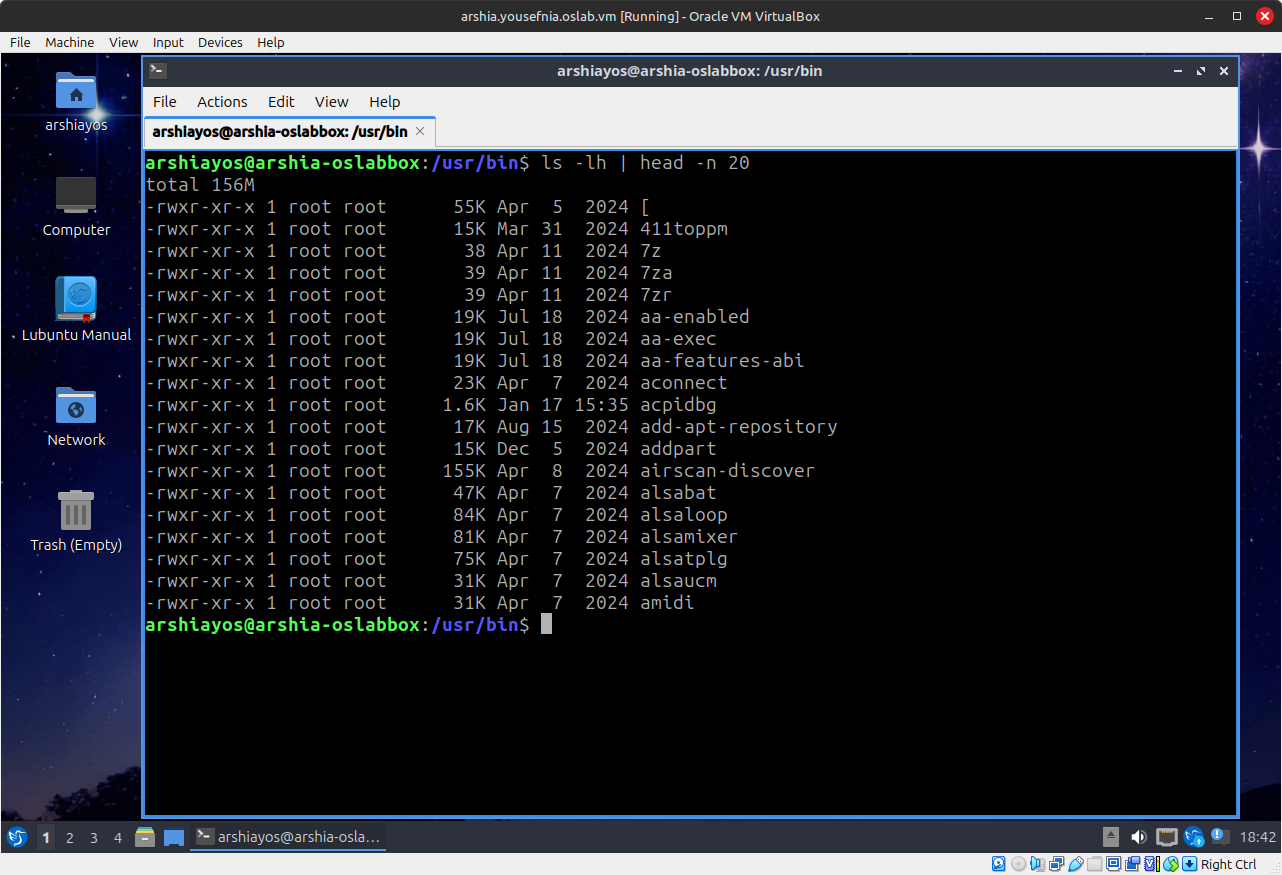
\includegraphics[width=0.8\textwidth]{report1-resources/23.png}
		\caption{حجم و سایر اطلاعات مربوط به فایل‌های \textenglish{/usr/bin/}}
	\end{figure}

        \item 
        در بخش‌های قبل، یک نمونه از کارکرد دستور 
        grep
        را دیدیم. برای اینکه بتوان عبارات جستجوی پیچیده‌تر را به آن داد، می‌توان از آپشن
        \textenglish{-E}
        استفاده کرد که با عبارت جستجو، مانند یک عبارت رجکس رفتار می‌کند. می‌دانیم در رجکس
        \textenglish{|}
        معادل
        or 
        است، پس مطابق شکل زیر، می‌توان به خواسته‌ی صورت آزمایش رسید.

        \begin{figure}[H]
		\centering
		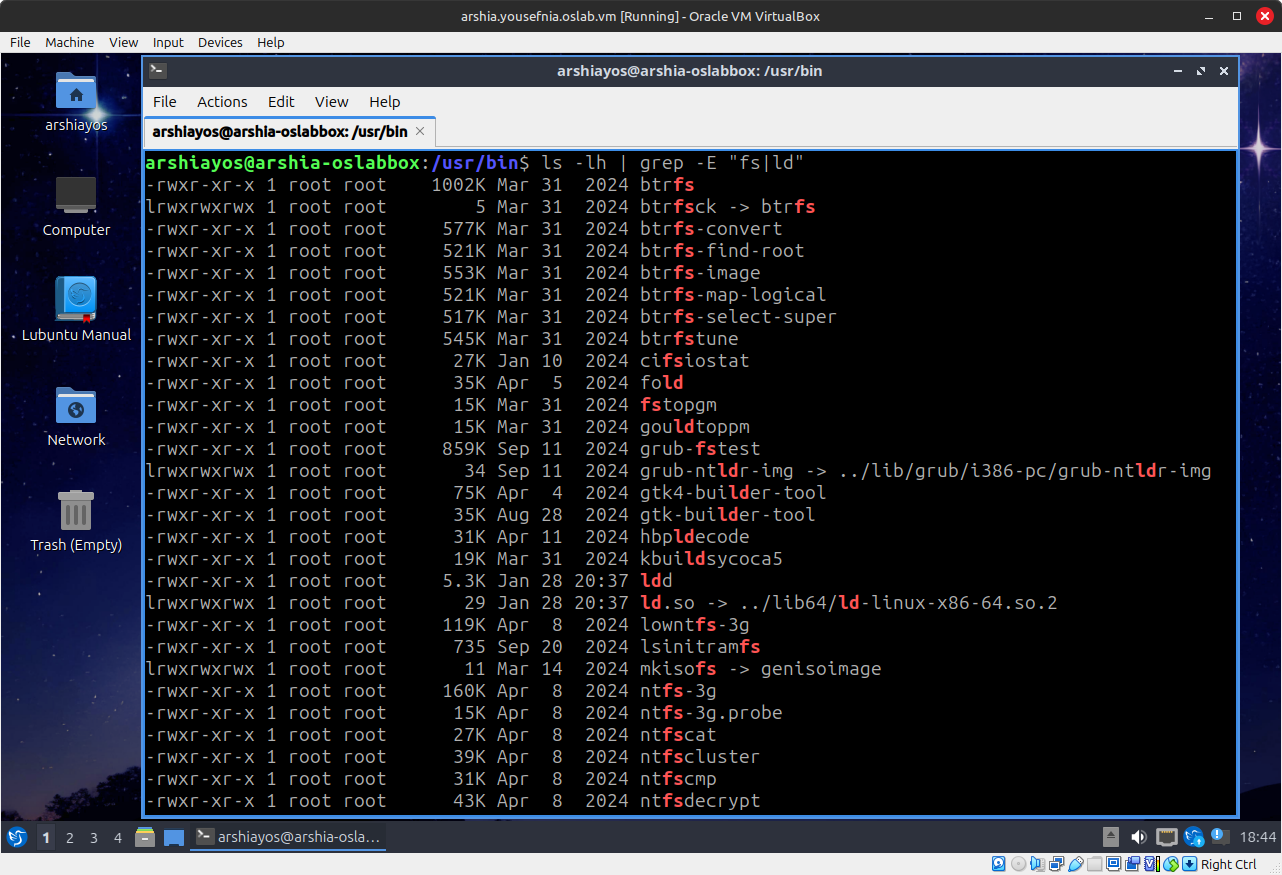
\includegraphics[width=0.8\textwidth]{report1-resources/24.png}
		\caption{نمایش لیست‌ فایل‌هایی که در آنها عبارات fs یا ld وجود دارد}
	\end{figure}
        
            
        \end{enumerate}


        \section{فعالیت‌ها}
        \begin{itemize}
            \item دستور \textenglish{cut}: 
            \cite{gnu-coreutils-cut}
            این دستور برای اینکه محتویات یک فایل را براساس یک کاراکتر یا عبارت در هر خط تقسیم کند و بخش‌های خاصی از آن را نمایش دهد. به بیان دیگر، این دستور فایل گفته شده را خط به خط بررسی کرده، و بسته به اینکه کدام آپشن‌ها استفاده می‌شوند، یا آن را با توجه به یک کاراکتر به چندین عبارت تقسیم کرده و عباراتی که کاربر می‌گوید را نشان می‌دهد، یا صرفا بایت‌ها یا کاراکترهایی که کاربر می‌گوید را در هر خط نشان می‌دهد.
            قالب کلی آن به این صورت است:

            \begin{english}
                cut [options] [file]
            \end{english}

            از آپشن‌های پرکاربر آن می‌توان به 
            \textenglish{-c}
            یا 
            \textenglish{-b}
            و همچنین
            \textenglish{-d}
            و 
            \textenglish{-f}
            اشاره کرد. دو آپشن آخر با هم می‌توانند در یک دستور قرار بگیرند، ولی سایر ترکیب آپشن‌ها نمی‌توانند.

            اگر از آپشن
            \textenglish{-c}
            یا 
            \textenglish{-b}
            استفاده شده باشد، کاربر می‌تواند به صورت یک لیست از چند بازه، شماره کاراکترها یا بایت‌هایی که می‌خواهد از هر خط نمایش داده شوند را تغیین کند.

            اگر از آپشن 
            \textenglish{-d}
            که جلوی آن باید حتما یک کاراکتر قرار بگیرد استفاده شود، هر خط از فایل توسط این کاراکتر به چند عبارت تقسیم شده، و شماره عباراتی که با آپشن
            \textenglish{-f}
            مشخص شده نمایش داده می‌شود. برای مثال اگر یک فایل 
            csv
            که اعضای هر خانه توسط کاما از هم جدا شده اند داشته باشیم، و بخواهیم ستون اول و سوم آن را مشاهده کنیم، می‌توانیم از این دستور استفاده کنیم:

            \begin{english}
                cut -d',' -f1,3 data.csv
            \end{english}

            \item دستور \textenglish{find}:
            این دستور برای جستجو بین فایل‌ها به کار می‌رود. قالب کلی آن به صورت 

            \begin{english}
                find [path] [expression]
            \end{english}

            است. بخش
            path
            مربوط به دایرکتوری جستجو است، و 
            expression
            جستجو بر اساس ویژگی‌های فایل است. از جمله آپشن‌هایی که در این بخش می‌توانند قرار بگیرند، می‌توان به 
            \textenglish{-name}
            اشاره کرد که براساس نام فایل جستجو را انجام می‌دهد، و قابلیت پشتیبانی از 
            wildcard
            را دارد، 
            \textenglish{-size}
            که براساس سایز فایل جستجو را انجام می‌دهد (برای مثال فایل‌های بزرگتر از 100 مگابایت)، 
            \textenglish{-mindepth}
            و
            \textenglish{-maxdepth}
            که حداقل و حداکثر عمق دایرکتوری را مشخص می‌کند، 
            \textenglish{-exec}
            که دستوری را روی فایل‌های پیدا شده اجرا می‌کند و ... اشاره کرد.

            \item دستور \textenglish{head}:
            \cite{gnu-coreutils-head}
            می‌تواند ابتدای یک فایل را پرینت کند. فرمت آن به صورت

            \begin{english}
                head [options] [file]
            \end{english}

            است، که از جمله آپشن‌های آن می‌توان به 
            \textenglish{-c}
            که تعداد بایت‌هایی که کاربر می‌خواهد از ابتدای فایل نمایش داده شود را مشخص می‌کند، و 
            \textenglish{-n}
            که تعداد خط‌هایی که کاربر می‌خواهد از ابتدای فایل نمایش داده شود مشخص می‌کند.

            \item دستور \textenglish{tail}:
            \cite{gnu-coreutils-tail}
            این دستور مانند دستور 
            head
            است، فقط با این تفاوت که انتهای فایل‌ها را نشان می‌دهد. آپشن‌هایی که در بالا برای 
            head
            معرفی کردیم، برای این دستور نیز به همان صورت وجود دارند، اما این دستور تعدادی آپشن اضافه‌تر هم دارد. مهم‌ترین آنها آپشن
            \textenglish{-f}
            است که با صورت بی‌درنگ و به طور دائم فایل را بررسی کرده و هرگاه چیزی به آن اضافه شود، آن را چاپ می‌کند.

            \item دستور \textenglish{touch}:
            \cite{gnu-coreutils-touch}
            این دستور برای ساخت فایل و/یا برای تغییر ویژگی‌های زمانی فایل‌ها (مانند 
            \textenglish{access time}
            یا
            \textenglish{modified time})
            به کار می‌رود. اگر آپشنی به کار نرود، این دستور فایلی را با 
            atime
            و
            mtime 
            فعلی می‌سازد. آپشن‌های
            \textenglish{-a}
            و
            \textenglish{-m}
            به ترتیب برای تغییر زمان
            atime
            و 
            mtime
            فایل‌هایی که وجود دارند نیز می‌توانند به کار بیایند.

            \item دستور \textenglish{wc}:
            \cite{gnu-coreutils-wc}
            این دستور برای شمارش تعداد خطوط/کلمات/کاراکترهای یک فایل می‌توان به کار برود. دستور آن به فرم

            \begin{english}
                wc [options] [file]
            \end{english}

            است. اگر آپشنی به کار نرود، به ترتیب تعداد خطوط، تعداد کلمات، و تعداد بایت‌های آن فایل را چاپ می‌کند. می‌توان به ترتیب از آپشن‌های
            \textenglish{-l}
            و 
            \textenglish{-w}
            و
            \textenglish{-c}
            استفاده کرد تا به ترتیب فقط یکی از آن سه عدد چاپ شود.

            این دستور دارای آپشن‌های دیگری نیز است که اطلاعات مشابهی را می‌دهند. برای مثال 
            \textenglish{-m}
            تعداد کاراکترهای فایل را نمایش می‌دهد، و 
            \textenglish{-L}
            طول بزرگترین خط را نشان می‌دهد.

            \item دستور \textenglish{kill}:
            \cite{gnu-coreutils-kill}
            این دستور سیگنال مورد نظر کاربر را برای پردازه‌ها می‌فرستد و  معمولا برای متوقف کردن پردازه‌ها به کار می‌رود. معمولا به فرمت زیر است:

            \begin{english}
                kill [-s signal | --signal signal | -signal] pid
            \end{english}

            برای مثال 
            \textenglish{kill 1234}
            سیگنال
            TERM
            را برای پردازه‌ی 1234 می‌فرستد. همچنین
            \textenglish{kill -9 1234}
            سیگنال 
            SIGKILL
            را برای پردازه می‌فرستد و آن را 
            \textenglish{force kill}
            می‌کند.
            
        \end{itemize}

        حال با کمک دستوراتی که از این بخش و بخش‌های قبل بررسی کردیم، خواسته‌های صورت آزمایش را انجام می‌دهیم.

        \begin{enumerate}
        \item برای این کار می‌توان از دستور
        wc
        با آپشن
        \textenglish{-l}
        استفاده کرد. یک نمونه از اجرای آن را در شکل زیر می‌توانید مشاهده کنید.

        \begin{figure}[H]
		\centering
		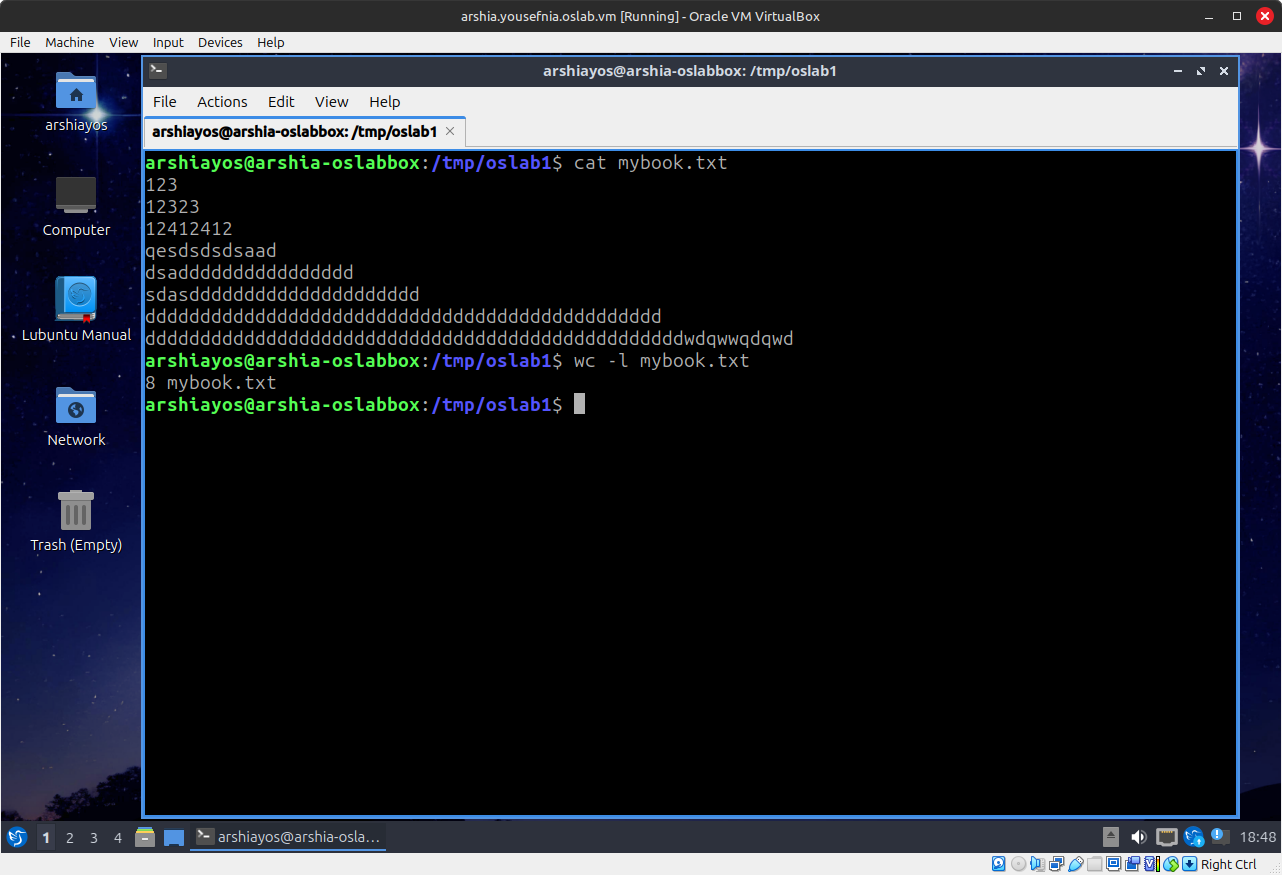
\includegraphics[width=0.8\textwidth]{report1-resources/25.png}
		\caption{پیدا کردن تعداد خطوط در یک فایل متنی}
	\end{figure}

        \item 
        می‌دانیم که دستور
        ls
        نام فایل‌ها را نمایش می‌دهد. اگر از آپشن
        \textenglish{-1}
        استفاده کنیم، در هر خط فقط نام یک فایل را نشان می‌دهد. همچنین اگر جلوی 
        ls
        عبارت
        \textenglish{A*}
        را قرار دهیم، به صورت 
        wildcard
        فقط فایل‌هایی که نامشان با 
        A
        شروع می‌شود را نشان می‌دهد. 
        پس اگر خروجی آن را به 
        wc
        تا تعداد خطوطش را محاسبه کند، به خواسته‌ی خود می‌رسیم. تنها نکته‌ای که باقی می‌ماند این است که 
        ls
        ممکن است ارور خروجی دهد. پس اگر خطاها را به ورودی 
        wc
        ندهیم، هیچگاه مشکلی پیش نمی‌آید. پس دستور
        \textenglish{ls -1 A* 2>/dev/null | wc -l}
        خواسته‌ی سوال را انجام می‌دهد. در شکل زیر می‌توان خروجی آن را مشاهده کرد.

        \begin{figure}[H]
		\centering
		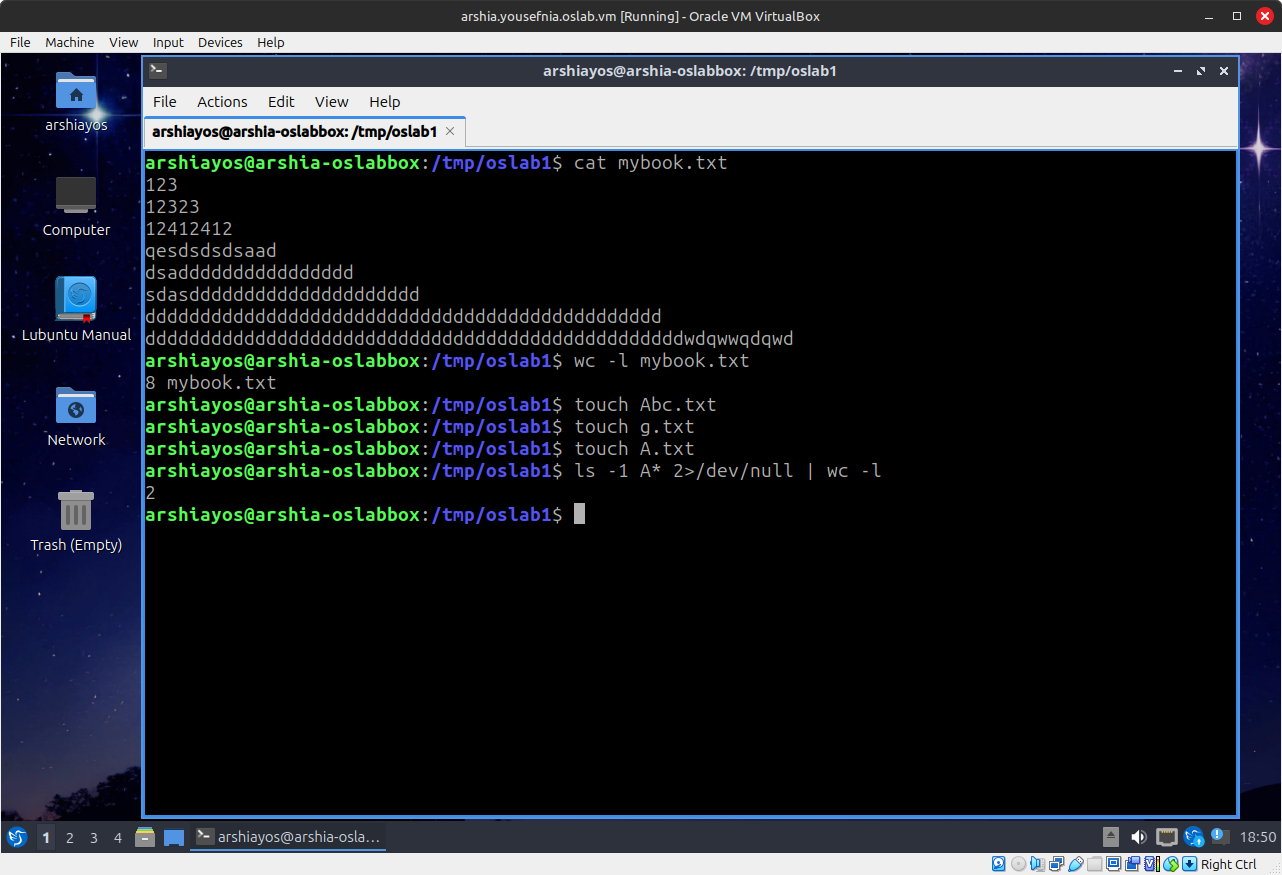
\includegraphics[width=0.8\textwidth]{report1-resources/26.png}
		\caption{پیدا کردن تعداد فایل‌هایی که با حرف A شروع می‌شوند}
	\end{figure}

        \item 
        همانطور که در بخش‌های قبل گفتیم، دستور 
        \textenglish{ls -lh}
        اطلاعاتی درمورد فایل‌ها (ازجمله حجمشان) را به ما می‌دهد. پس با دستور 
        \textenglish{ls -lh mybook.txt}
        می‌توانیم به خواسته‌ی خود برسیم. 

        \begin{figure}[H]
		\centering
		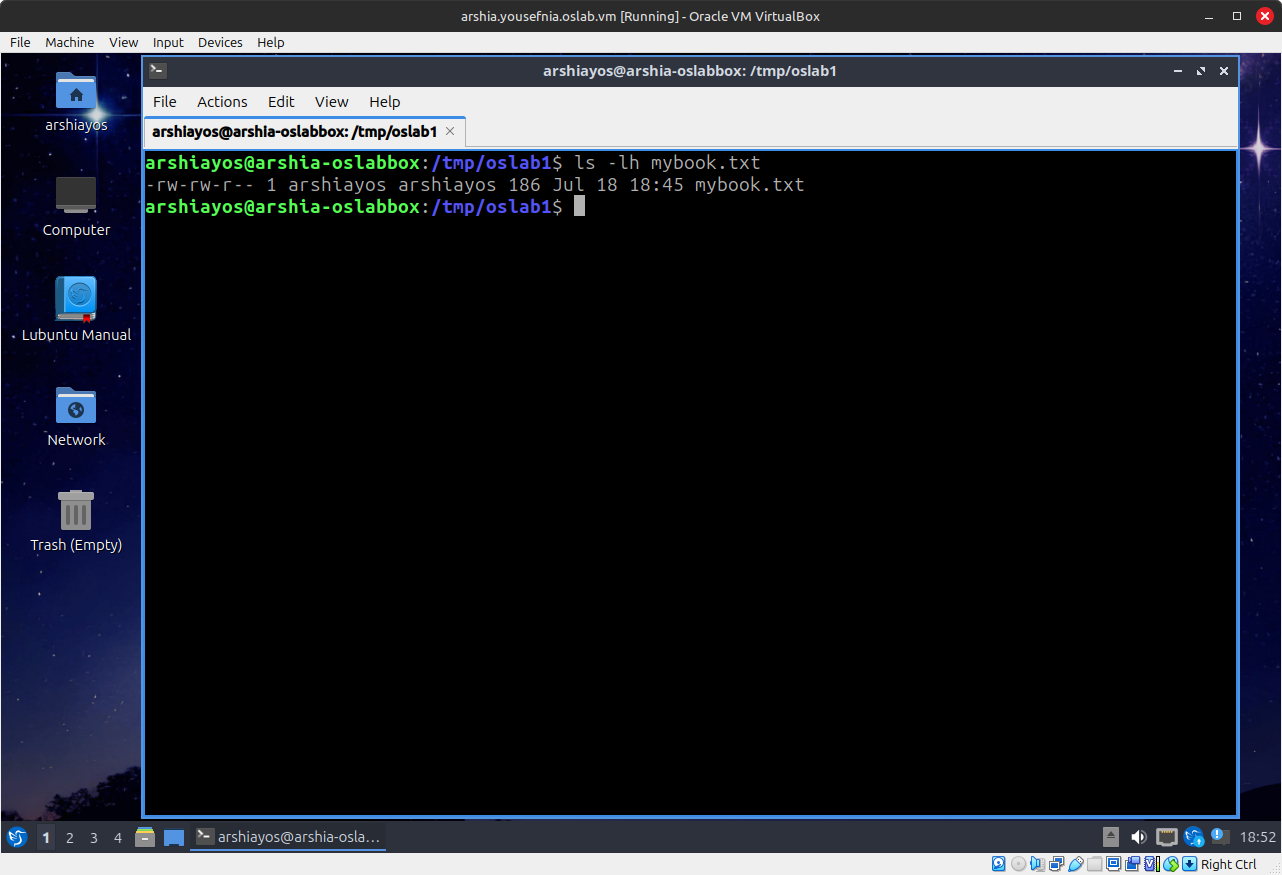
\includegraphics[width=0.8\textwidth]{report1-resources/27.png}
		\caption{نمایش حجم یک فایل}
	\end{figure}
        \end{enumerate}

        \subsection{اعمال تغییرات و کامپایل مجدد هسته‌ی سیستم عامل}
        ابتدا با دستور
        \textenglish{uname -r}
        نسخه‌ی هسته‌ی فعلی را نشان می‌دهیم.

        \begin{figure}[H]
		\centering
		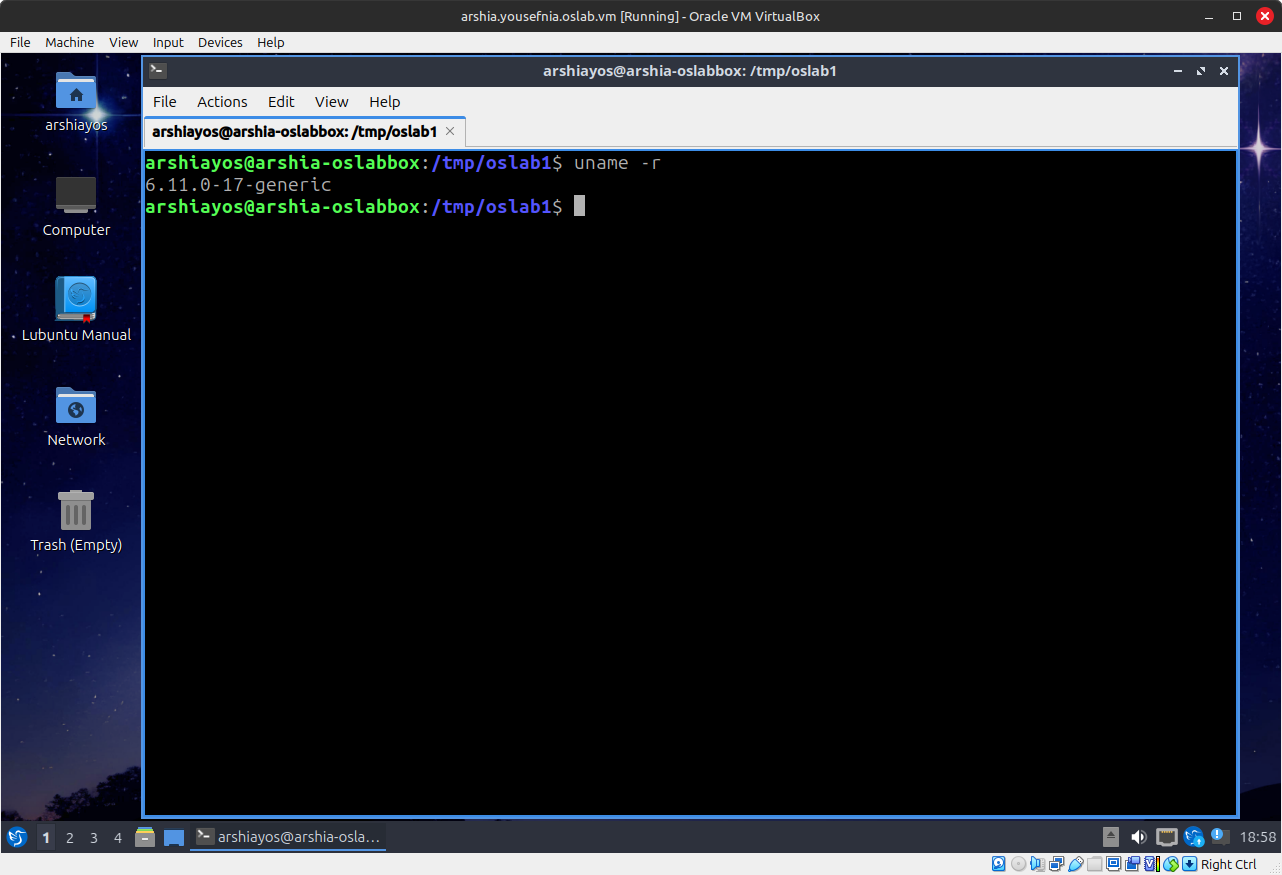
\includegraphics[width=0.8\textwidth]{report1-resources/28.png}
		\caption{نمایش نسخه‌ی هسته قبل از کامپایل}
	\end{figure}

        \begin{enumerate}
        \item مطابق شکل زیر، کد منبع هسته را دریافت می‌کنیم.
        
        \begin{figure}[H]
		\centering
		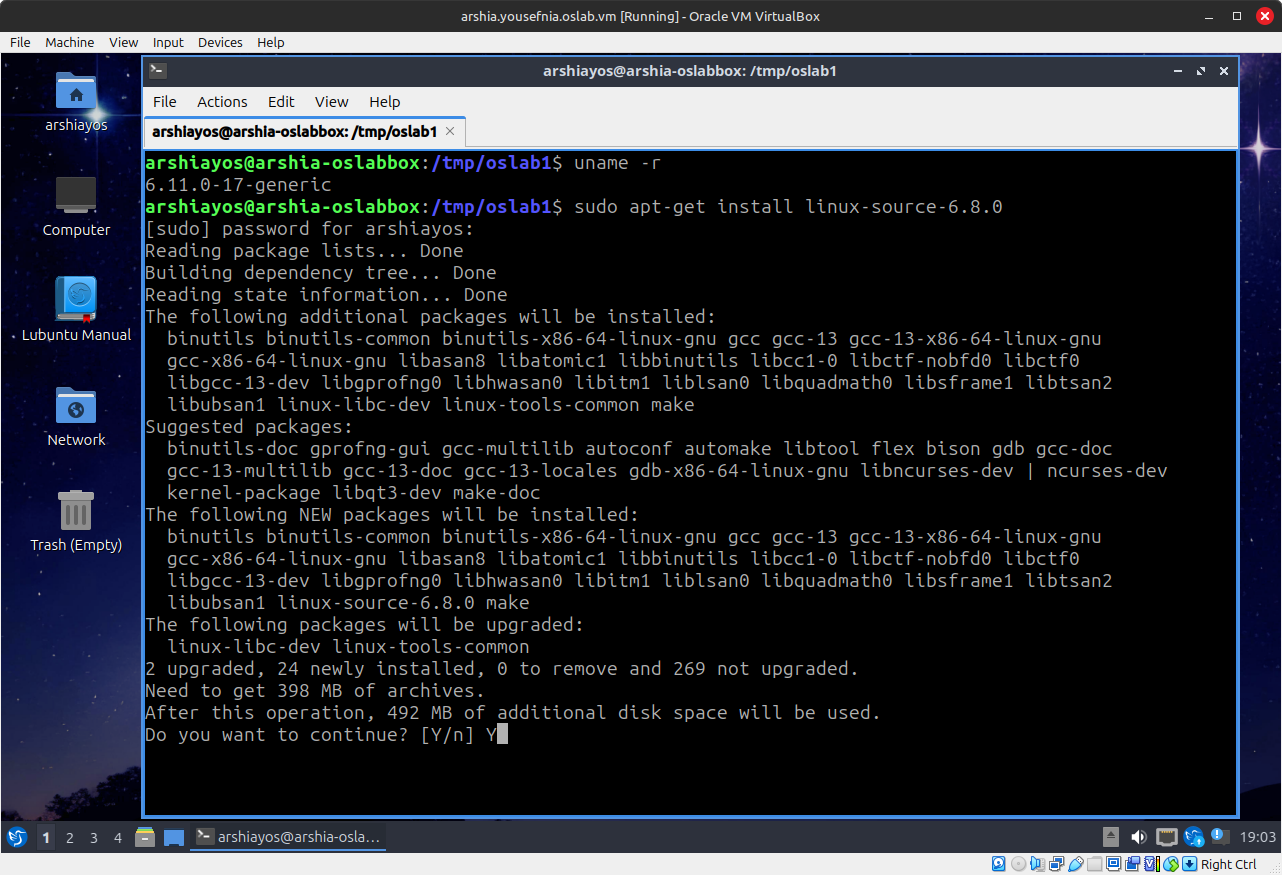
\includegraphics[width=0.8\textwidth]{report1-resources/29.png}
		\caption{دریافت کد هسته}
	\end{figure}

        سپس  مطابق دو شکل زیر، ابزارهای لازم برای کامپایل هسته را دریافت می‌کنیم.

        \begin{figure}[H]
		\centering
		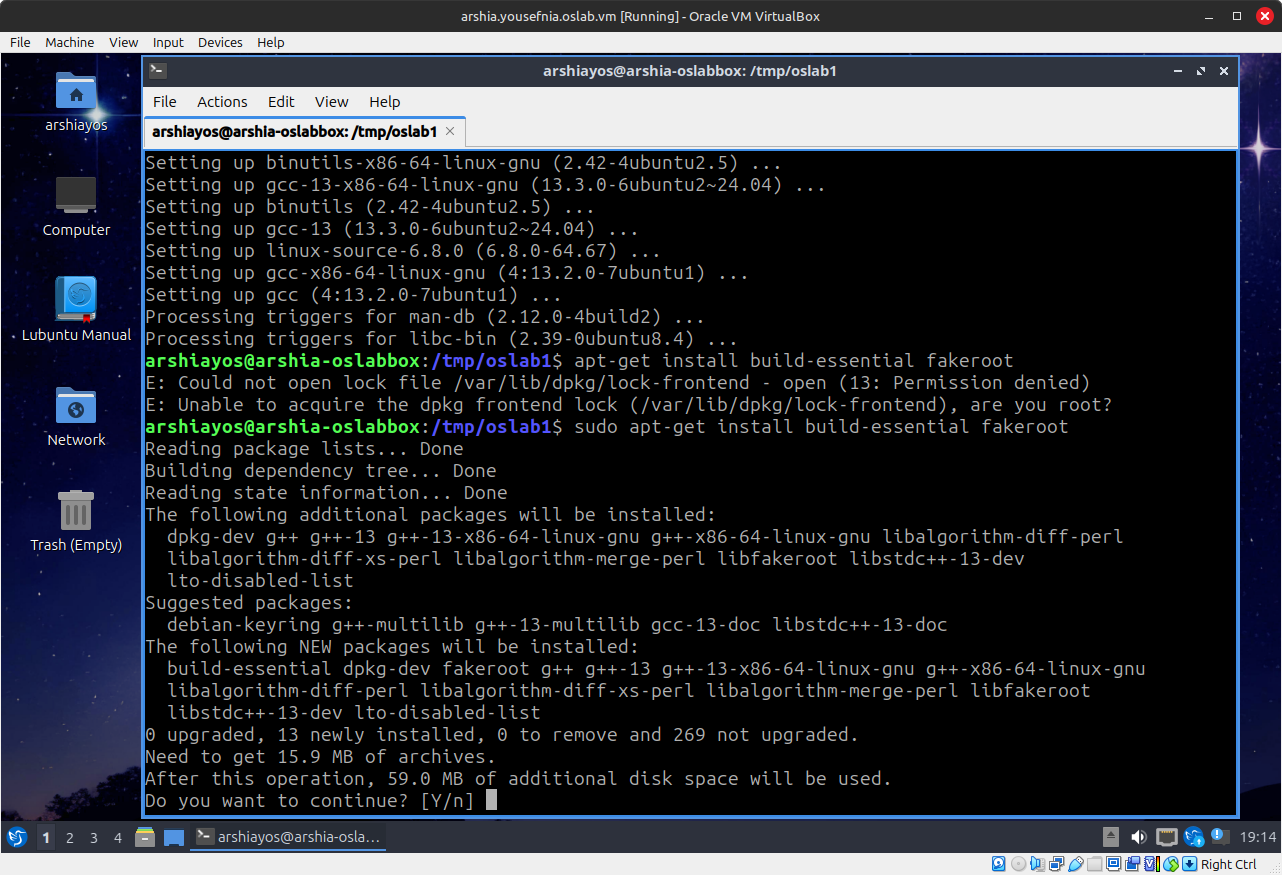
\includegraphics[width=0.8\textwidth]{report1-resources/33.png}
		\caption{دریافت ابزارهای لازم برای کامپایل هسته (بخش اول)}
	\end{figure}

        \begin{figure}[H]
		\centering
		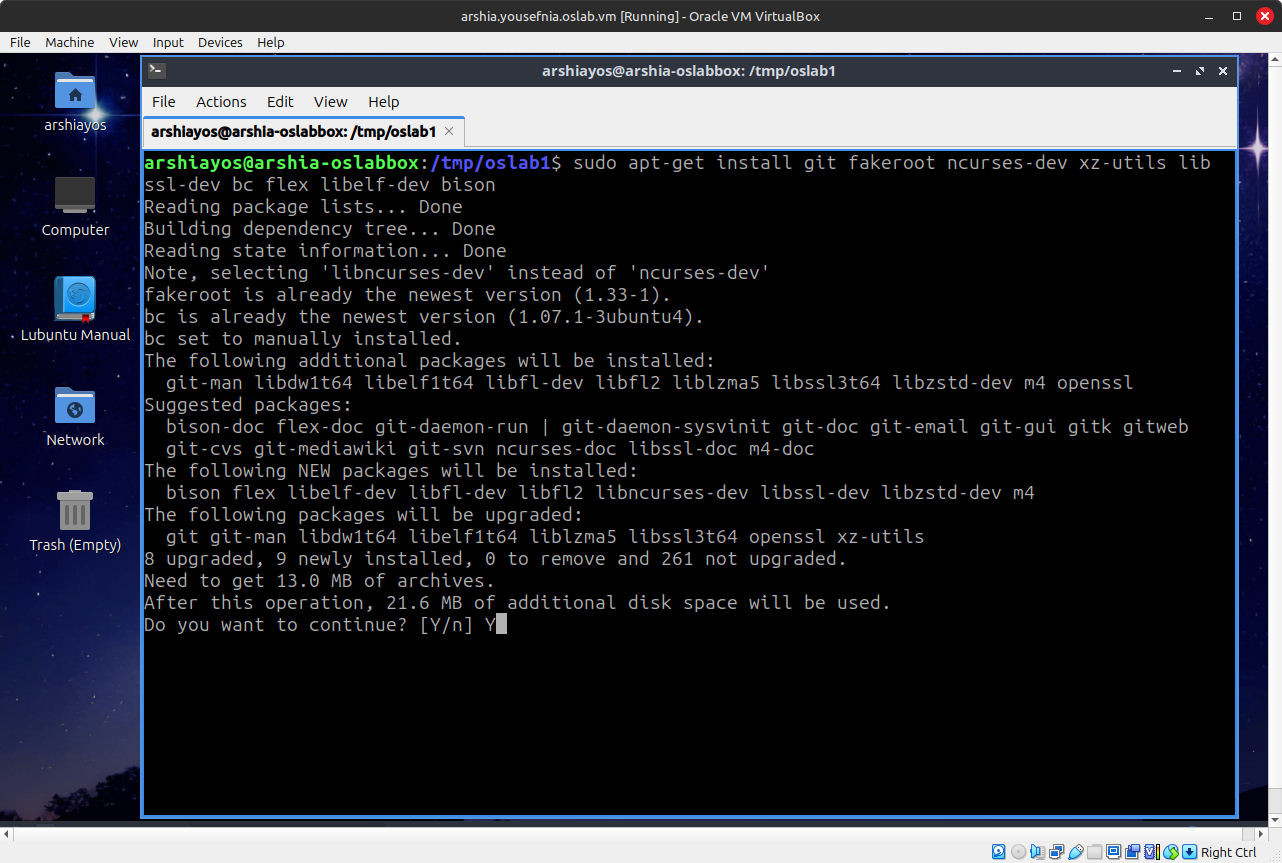
\includegraphics[width=0.8\textwidth]{report1-resources/34.png}
		\caption{دریافت ابزارهای لازم برای کامپایل هسته (بخش دوم)}
	\end{figure}

        \item سپس مطابق شکل زیر، کدهای هسته را در یک  پوشه بازگشایی می‌کنیم.

        \begin{figure}[H]
		\centering
		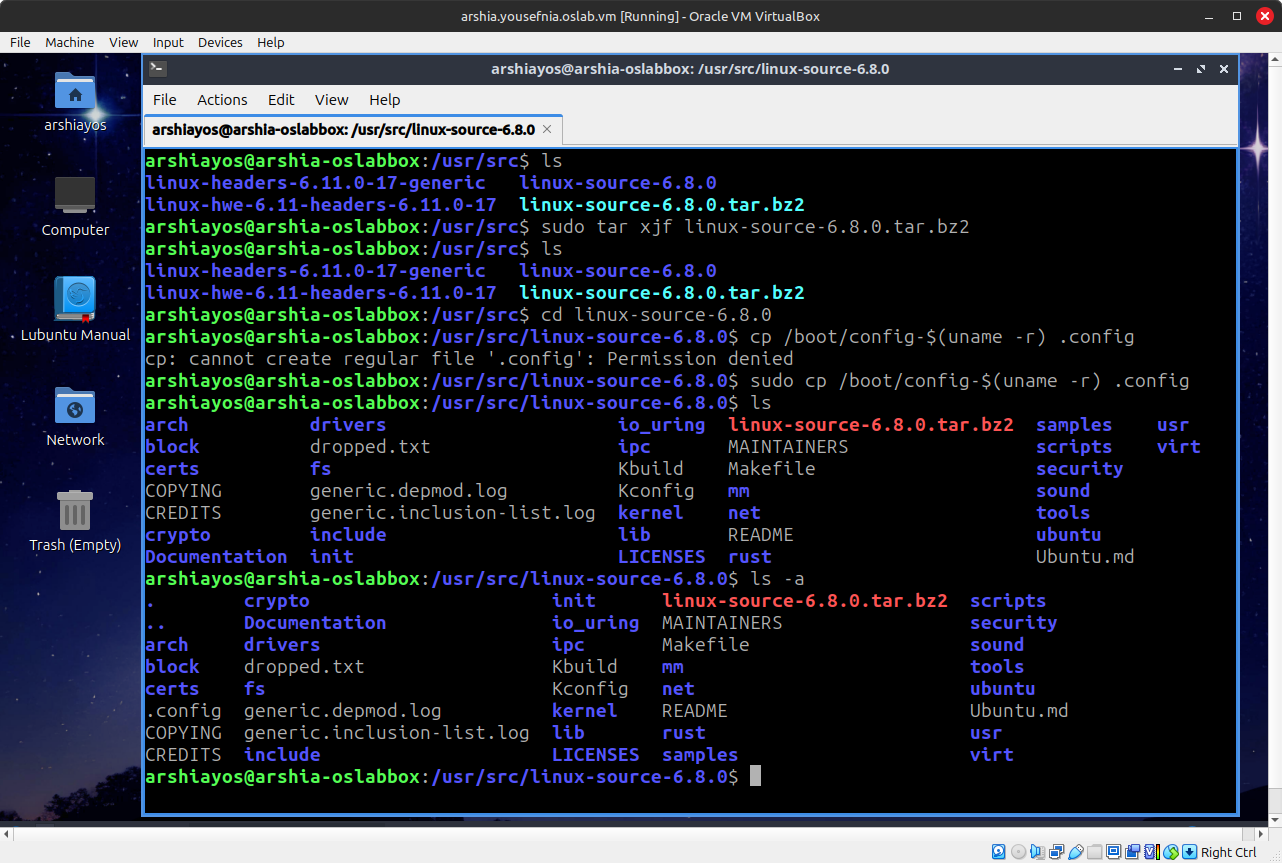
\includegraphics[width=0.8\textwidth]{report1-resources/36.png}
		\caption{بازگشایی کدهای هسته و ورود به آن}
	\end{figure}
        \end{enumerate}

        \subsection{فعالیت‌ها (ادامه‌ی کامپایل)}
        در این بخش توضیح کوتاهی درمورد ادامه‌ی مراحل کامپایل داده و شکل‌های مربوط به آن بخش را می‌گذاریم. 

        در ادامه‌ی مراحل کامپایل، ابتدا باید 
        configuration
        سیستم عامل را برای کامپایل تنظیم کنیم. یکی از روش‌های پر استفاده، دستور 
        \textenglish{make menuconfig}
        است که دارای محیط کاربری برای تنظیم 
        config
        است.

        \begin{figure}[H]
		\centering
		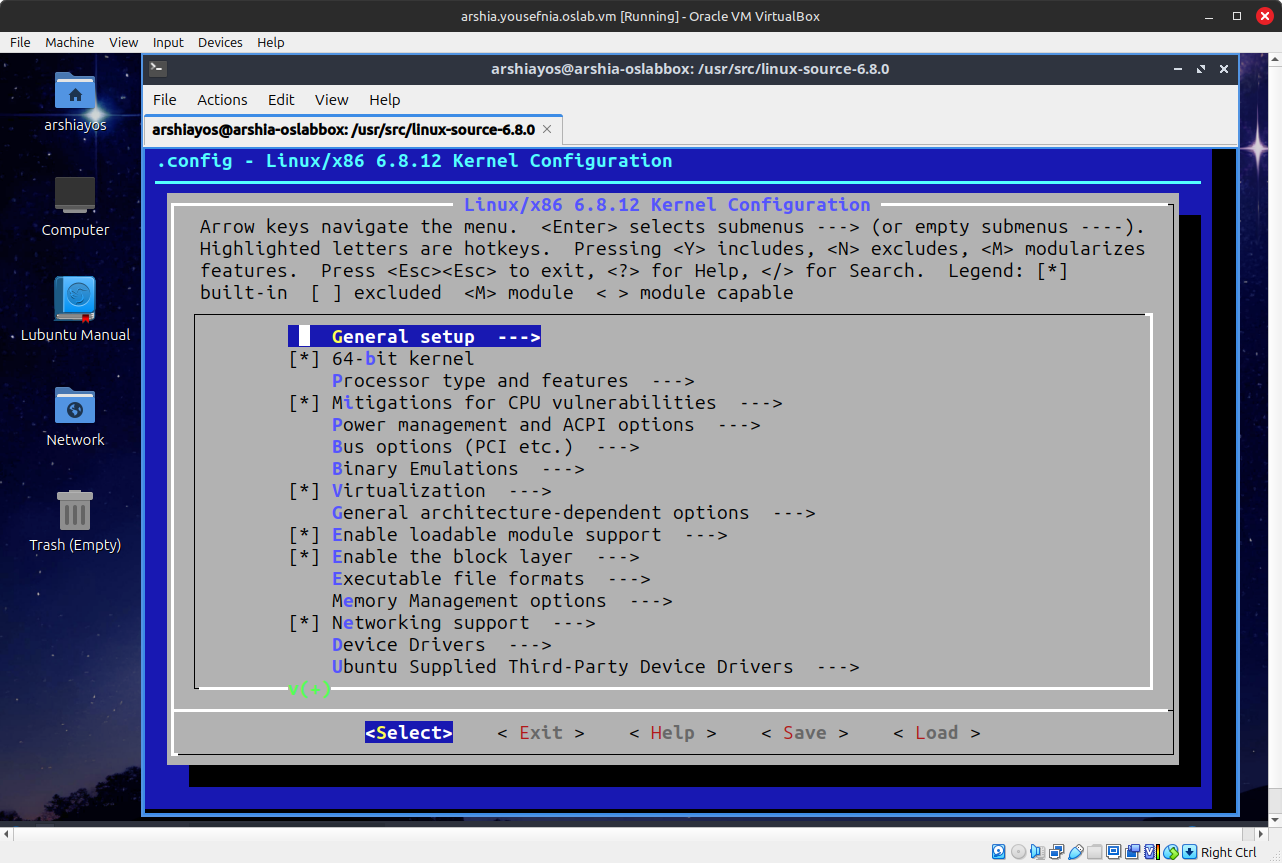
\includegraphics[width=0.8\textwidth]{report1-resources/37.png}
		\caption{محیط \textenglish{make menuconfig}}
	\end{figure}

        اما از آنجایی که ما صرفا داریم ورژن هسته‌ی لینوکس را تغییر می‌دهیم، یک روش ساده‌تر، استفاده از 
        \textenglish{make oldconfig}
        است که از 
        config
        قبلی استفاده می‌کند و فقط درباره‌ی موارد جدید 
        config
        از کاربر سوال می‌پرسد. ما هم از 
        config
        قبلی یک 
        backup
        گرفته و با این دستور، فایل
        \textenglish{.config}
        را آماده می‌کنیم.

        \begin{figure}[H]
		\centering
		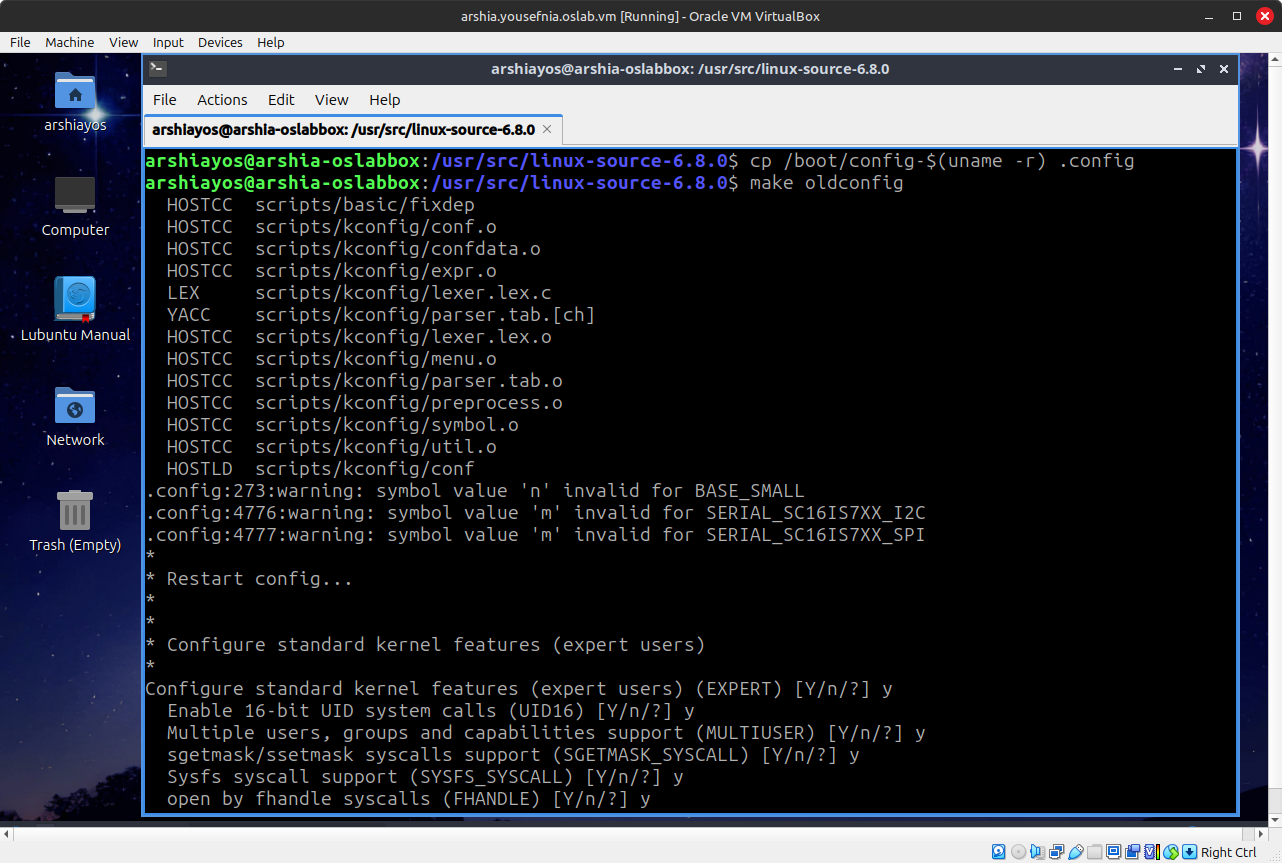
\includegraphics[width=0.8\textwidth]{report1-resources/40.png}
		\caption{استفاده از \textenglish{make oldconfig}}
	\end{figure}

        سپس با دستور 
        \textenglish{make -j\$(nproc)}
        هسته را کامپایل می‌کنیم.

        \begin{figure}[H]
		\centering
		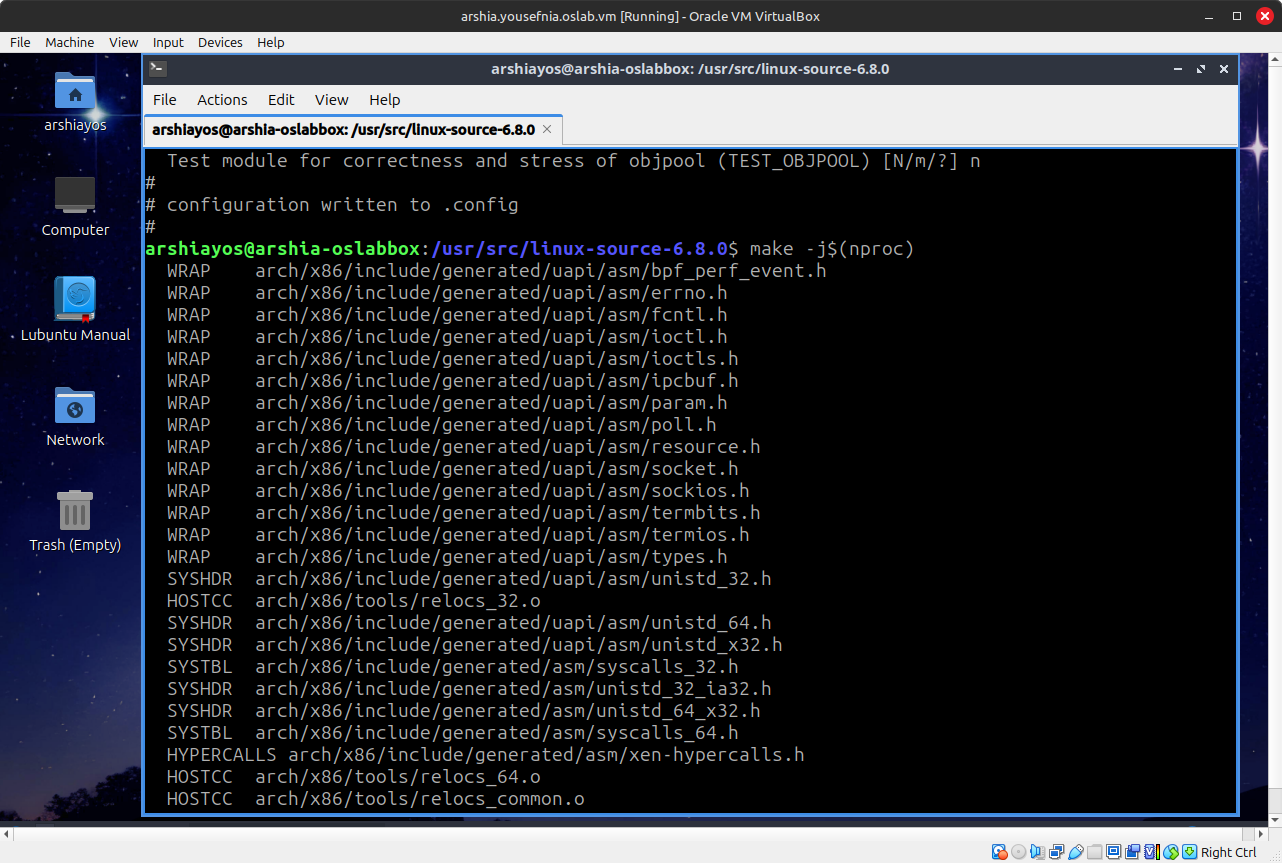
\includegraphics[width=0.8\textwidth]{report1-resources/42.png}
		\caption{کامپایل مجدد هسته}
	\end{figure}

        پس از کامپایل، باید هسته‌ی جدید را نصب کنیم. برای این کار ابتدا ماژول‌ها را با دستور
        \textenglish{make modules\_install}
        نصب کرده و سپس با دستور
        \textenglish{make install}
        می‌توان
        image
        هسته را نصب کرد.

        \begin{figure}[H]
		\centering
		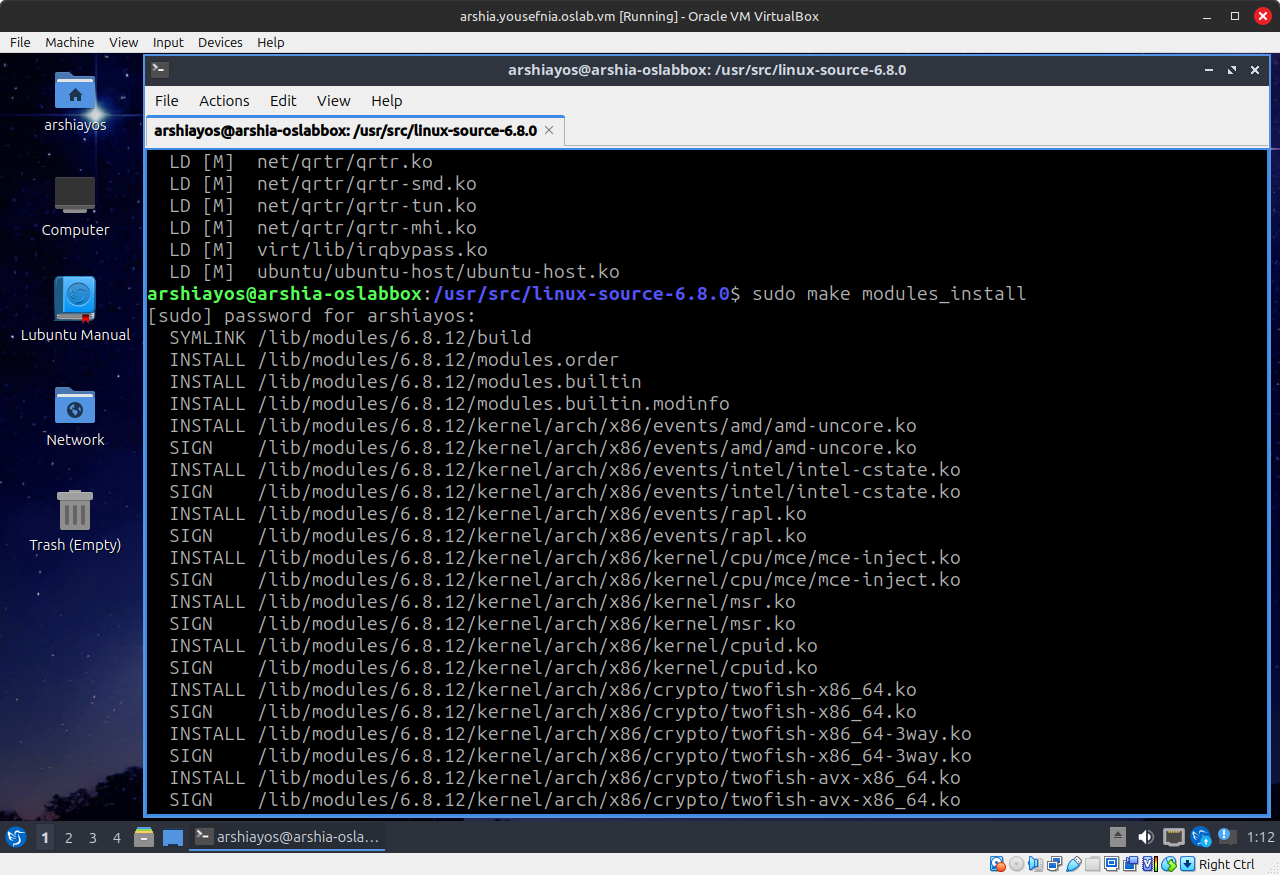
\includegraphics[width=0.8\textwidth]{report1-resources/51.png}
		\caption{نصب ماژول‌های هسته}
	\end{figure}

        \begin{figure}[H]
		\centering
		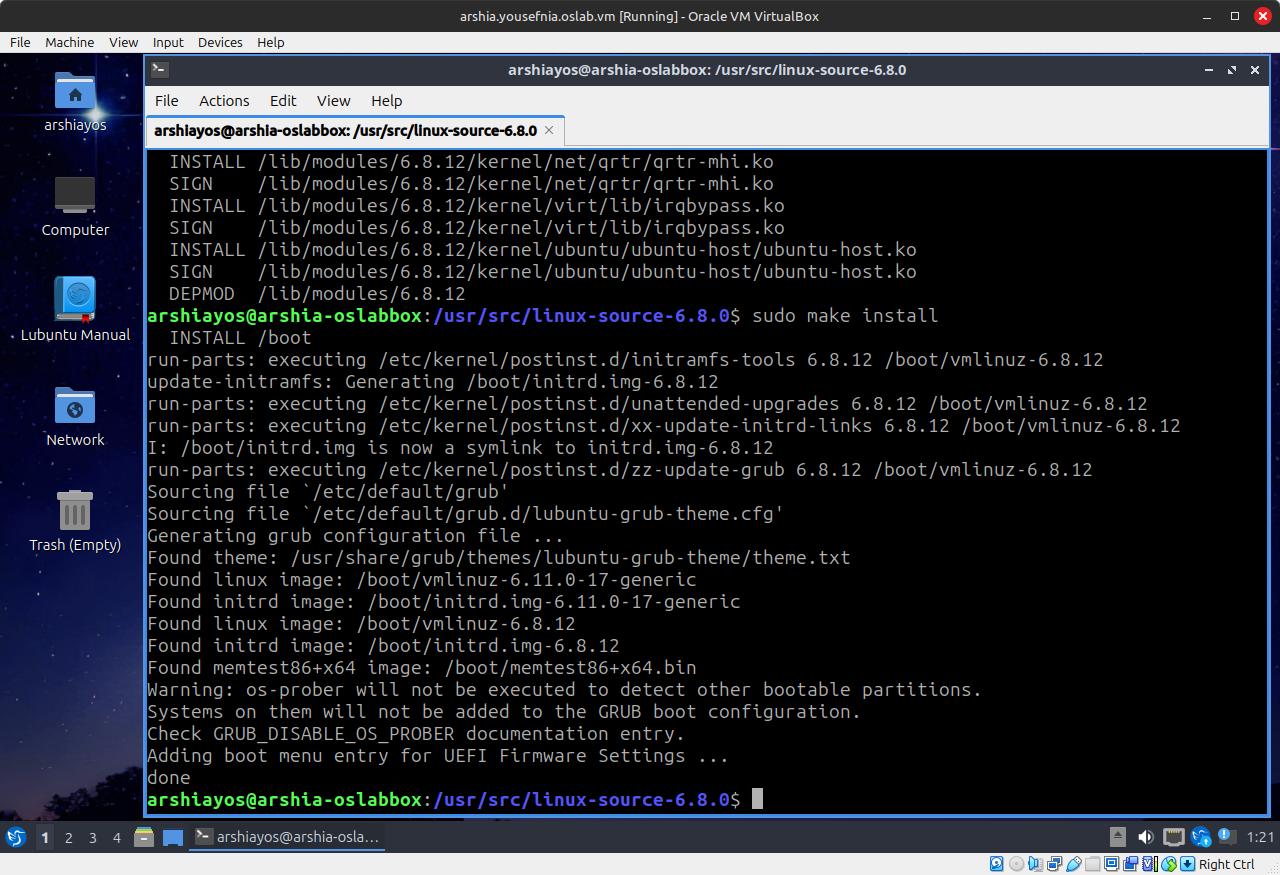
\includegraphics[width=0.8\textwidth]{report1-resources/53.png}
		\caption{نصب image هسته}
	\end{figure}

        درنهایت باید سیستم را
        reboot
        کنیم. هنگام 
        boot
        کردن، باید نسخه‌ای که به تازگی کامپایل کرده‌ایم را انتخاب کرده و اجرا کنیم.

        \begin{figure}[H]
		\centering
		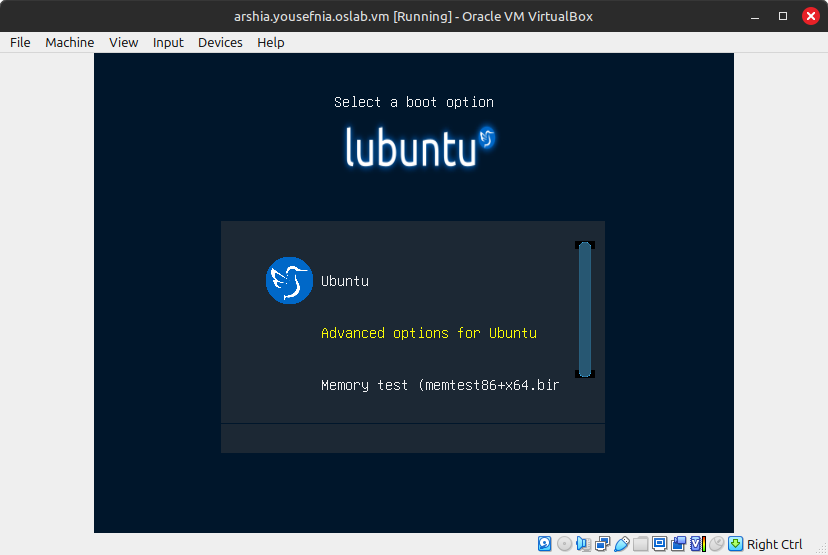
\includegraphics[width=0.8\textwidth]{report1-resources/54.png}
		\caption{انتخاب نسخه‌ی جدید هنگام boot}
	\end{figure}

    \begin{figure}[H]
		\centering
		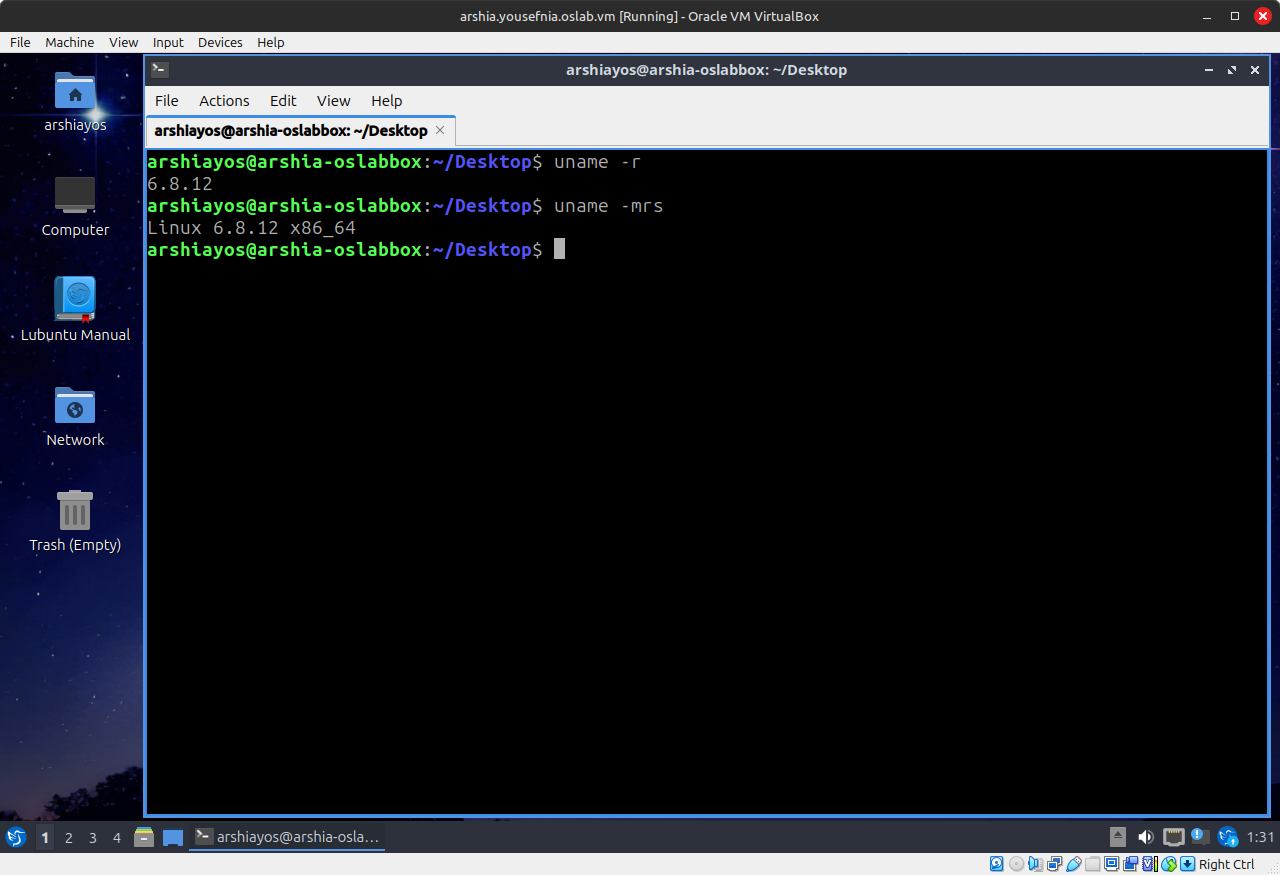
\includegraphics[width=0.8\textwidth]{report1-resources/56.png}
		\caption{بررسی درستی کامپایل و نصب با دستور \textenglish{uname -r}}
	\end{figure}
	
	% ==============================
	% References
	% ==============================
	\newpage
	\begin{LTR}
		\begin{english}
\printbibliography[title={مراجع}]
\end{english}
	\end{LTR}

	
\end{document}

